%\documentclass[handout,xcolor=pdftex,dvipsnames,table,mathserif]{beamer}
\documentclass[xcolor=pdftex,dvipsnames,table,mathserif]{beamer}
%\usepackage{subfigure}
\usepackage{amsbsy}
\usepackage{tikz}
\usetikzlibrary{arrows}
\usepackage{amsmath,graphicx,dsfont,color}
\usepackage{amsfonts}
\usepackage{amssymb}
\usepackage{array}

\usepackage{subfig}

% makes the subfig package work
\makeatletter
\let\@@magyar@captionfix\relax
\makeatother

% subfigure counter resets every frame
\makeatletter
\@addtoreset{subfigure}{framenumber}
\makeatother

% First author and year
\bibliographystyle{apalike}

% This sets the list items of the bibliography to the same symbol used for citation.
\setbeamertemplate{bibliography item}{\insertbiblabel}

% This avoids extralines for different entries
\setbeamertemplate{bibliography entry title}{}
\setbeamertemplate{bibliography entry location}{}
\setbeamertemplate{bibliography entry note}{}

\DeclareMathOperator*{\argmin}{arg\,min}
\DeclareMathOperator*{\argmax}{arg\,max}
%Definitiona

\newcommand{\x}{\mathbf{x}}
\newcommand{\X}{\mathbf{X}}
\newcommand{\W}{\mathbf{W}} %Weight
\newcommand{\bais}{\mathbf{b}}%Bais
\newcommand{\act}{\texttt{g}}%Activation
\newcommand{\loss}{L}
\newcommand{\pdata}{\hat{p}_{\texttt{data}}}
\newcommand{\nsize}{N}
\newcommand{\nfeatures}{P}
\newcommand{\param}{\boldsymbol{\theta}}
\newcommand{\featmap}{\boldsymbol{\phi}}
\newcommand{\EV}{\mathbb{E}}







\usepackage{physics}

\graphicspath{{../graphics/}}

\AtBeginSection[]{
  \begin{frame}{Contents}
    \tableofcontents[currentsection, hideothersubsections]
  \end{frame}
}

\AtBeginSubsection[]{
  \begin{frame}{Contents}
    \tableofcontents[currentsection, subsectionstyle=show/shaded/hide]
  \end{frame}
}

\setbeamertemplate{footline}[frame number]{}
\setbeamertemplate{navigation symbols}{}
\setbeamertemplate{section in toc}[square]
\setbeamertemplate{items}[square]

%% For image credits on image bottom right
\usepackage[absolute,overlay]{textpos}
\setbeamercolor{framesource}{fg=gray}
\setbeamerfont{framesource}{size=\tiny}
\newcommand{\source}[1]{\begin{textblock*}{4cm}(8.7cm,8.6cm)
    \begin{beamercolorbox}[ht=0.5cm,right]{framesource}
      \usebeamerfont{framesource}\usebeamercolor[fg]{framesource} Credits: {#1}
    \end{beamercolorbox}
\end{textblock*}}

\title{Fully convolutional neural networks}
\author{E. Decencière}
\date{MINES ParisTech\\
  PSL Research University\\
  Center for Mathematical Morphology
}
\titlegraphic{
\includegraphics[height=1.7cm]{../graphics/logoemp}}

\useinnertheme{rounded}
\usecolortheme{rose}

%%%%%%%%%%%%%%%%%%%%%%%%%%%%%%%%%%%%%%%%%%%%%%%%%%%%%%%
%%%%%%%%%%%%%%%%%%%%%%%%%%%%%%%%%%%%%%%%%%%%%%%%%%%%%%%

\begin{document}

\frame{\titlepage}

\frame{
  \frametitle{Contents}
  \tableofcontents[hidesubsections]
}

%%%%%%%%%%%%%%%%%%%%%%%%%%%%%%%%%%%%%%%%%%%%%%%%%%
%%%%%%%%%%%%%%%%%%%%%%%%%%%%%%%%%%%%%%%%%%%%%%%%%%
\section{Introduction}


%%%%%%%%%%%%%%%%%%%%%%%%%%%%%%%%%%%%
%% \begin{frame}{Recall from yesterday: image classification with NN}

%%   \begin{columns}

%%     \begin{column}{.5\textwidth}
%%       \begin{figure}[ht]
%%         \centering
%%         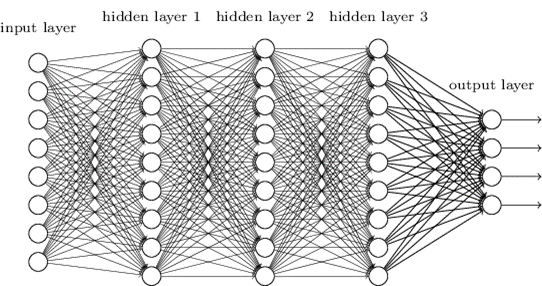
\includegraphics[width=\textwidth]{network.png}\\
%%         Simple fully-connected neural network
%%       \end{figure}
%%     \end{column}

%%     \begin{column}{.5\textwidth}
%%       The cross-entropy loss function used for classification tasks:
%%       \[
%%       \loss(\param) = \sum\limits_{i=1}^n H(\y, f(\x_i, \param))
%%       \]

%%       where the cross-entropy $H$ is defined as:

%%       \[
%%       H(\y, \hat{\y}) = -\sum\limits_{i=1}^q \y_i \log( \hat{\y_i})
%%       \]
%%     \end{column}
%%   \end{columns}

%% \end{frame}


%%%%%%%%%%%%%%%%%%%%%%%%%%%%%%%%%%%%
\begin{frame}{Learning image transformations}

  \begin{itemize}
  \item An image classification task is a function from the set of considered images into a set of labels
      \begin{figure}
      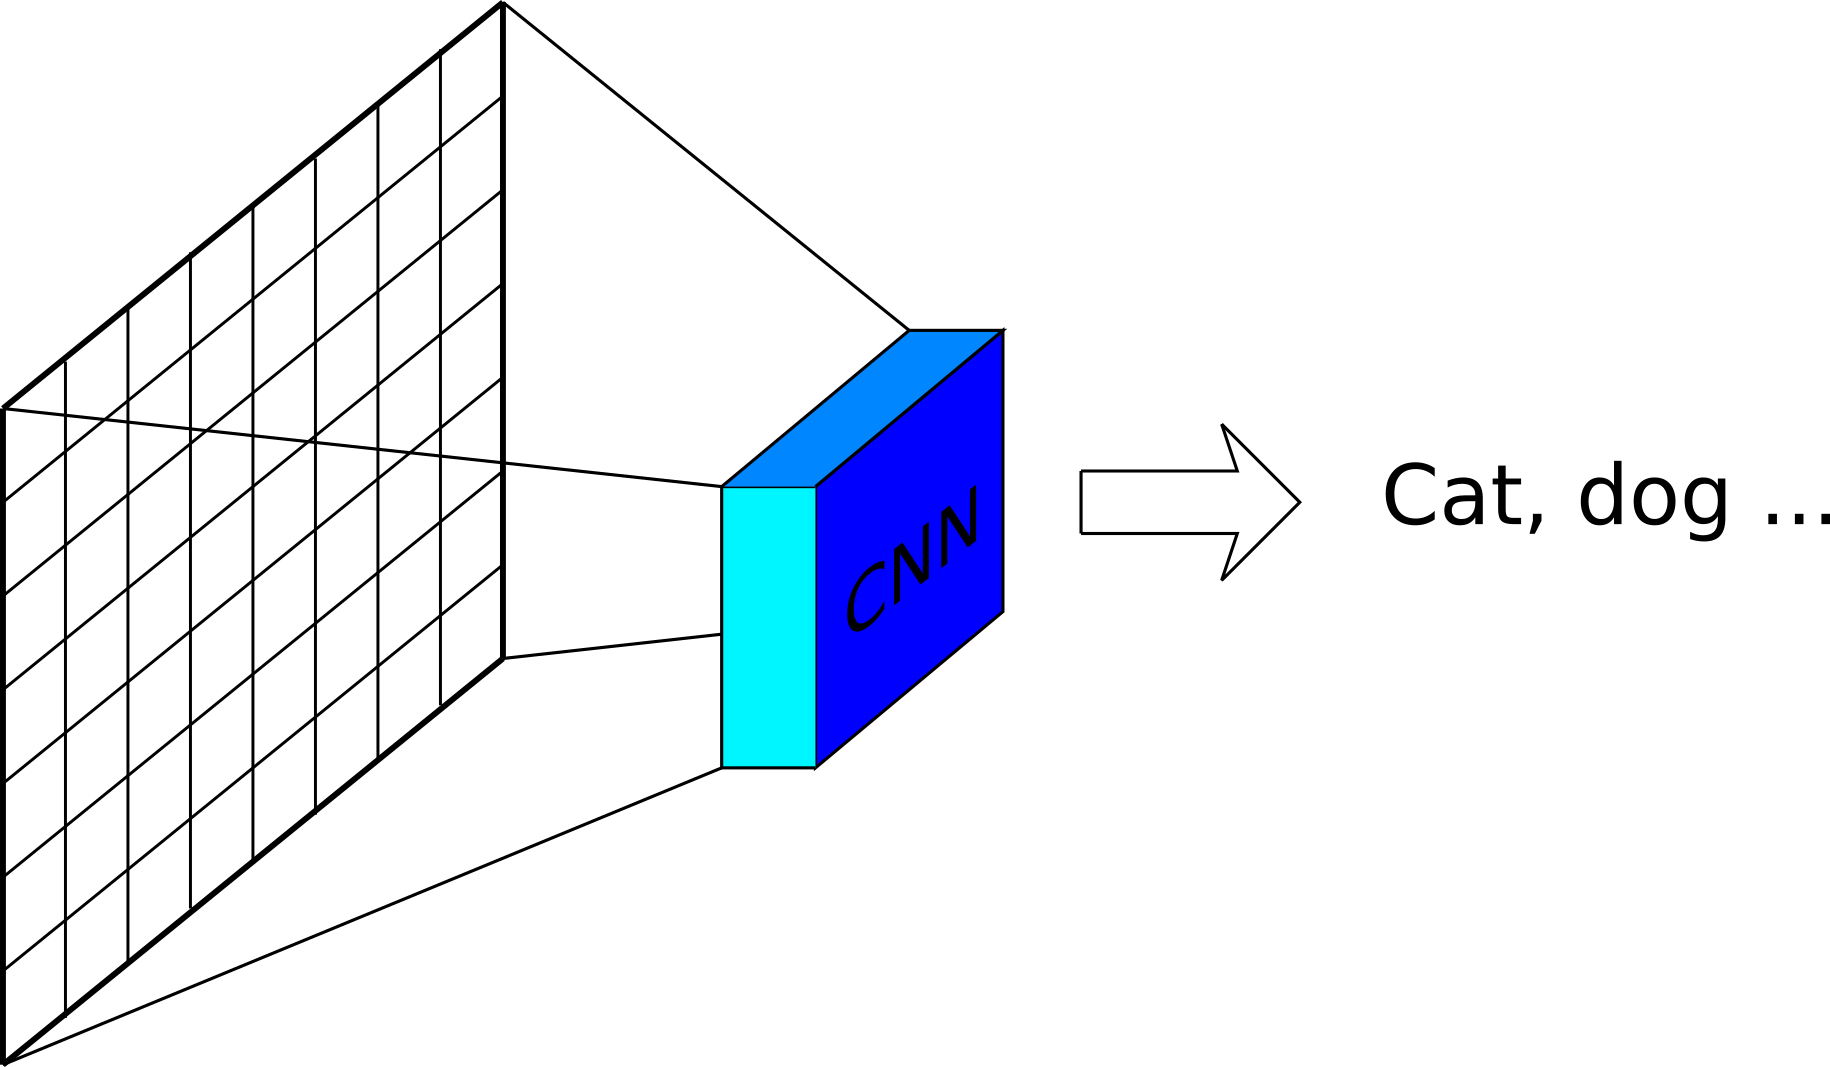
\includegraphics[width=0.40\textheight]{image_classif.png}
      \end{figure}
  \item In many applications, we want to transform an image into another image
      \begin{figure}
      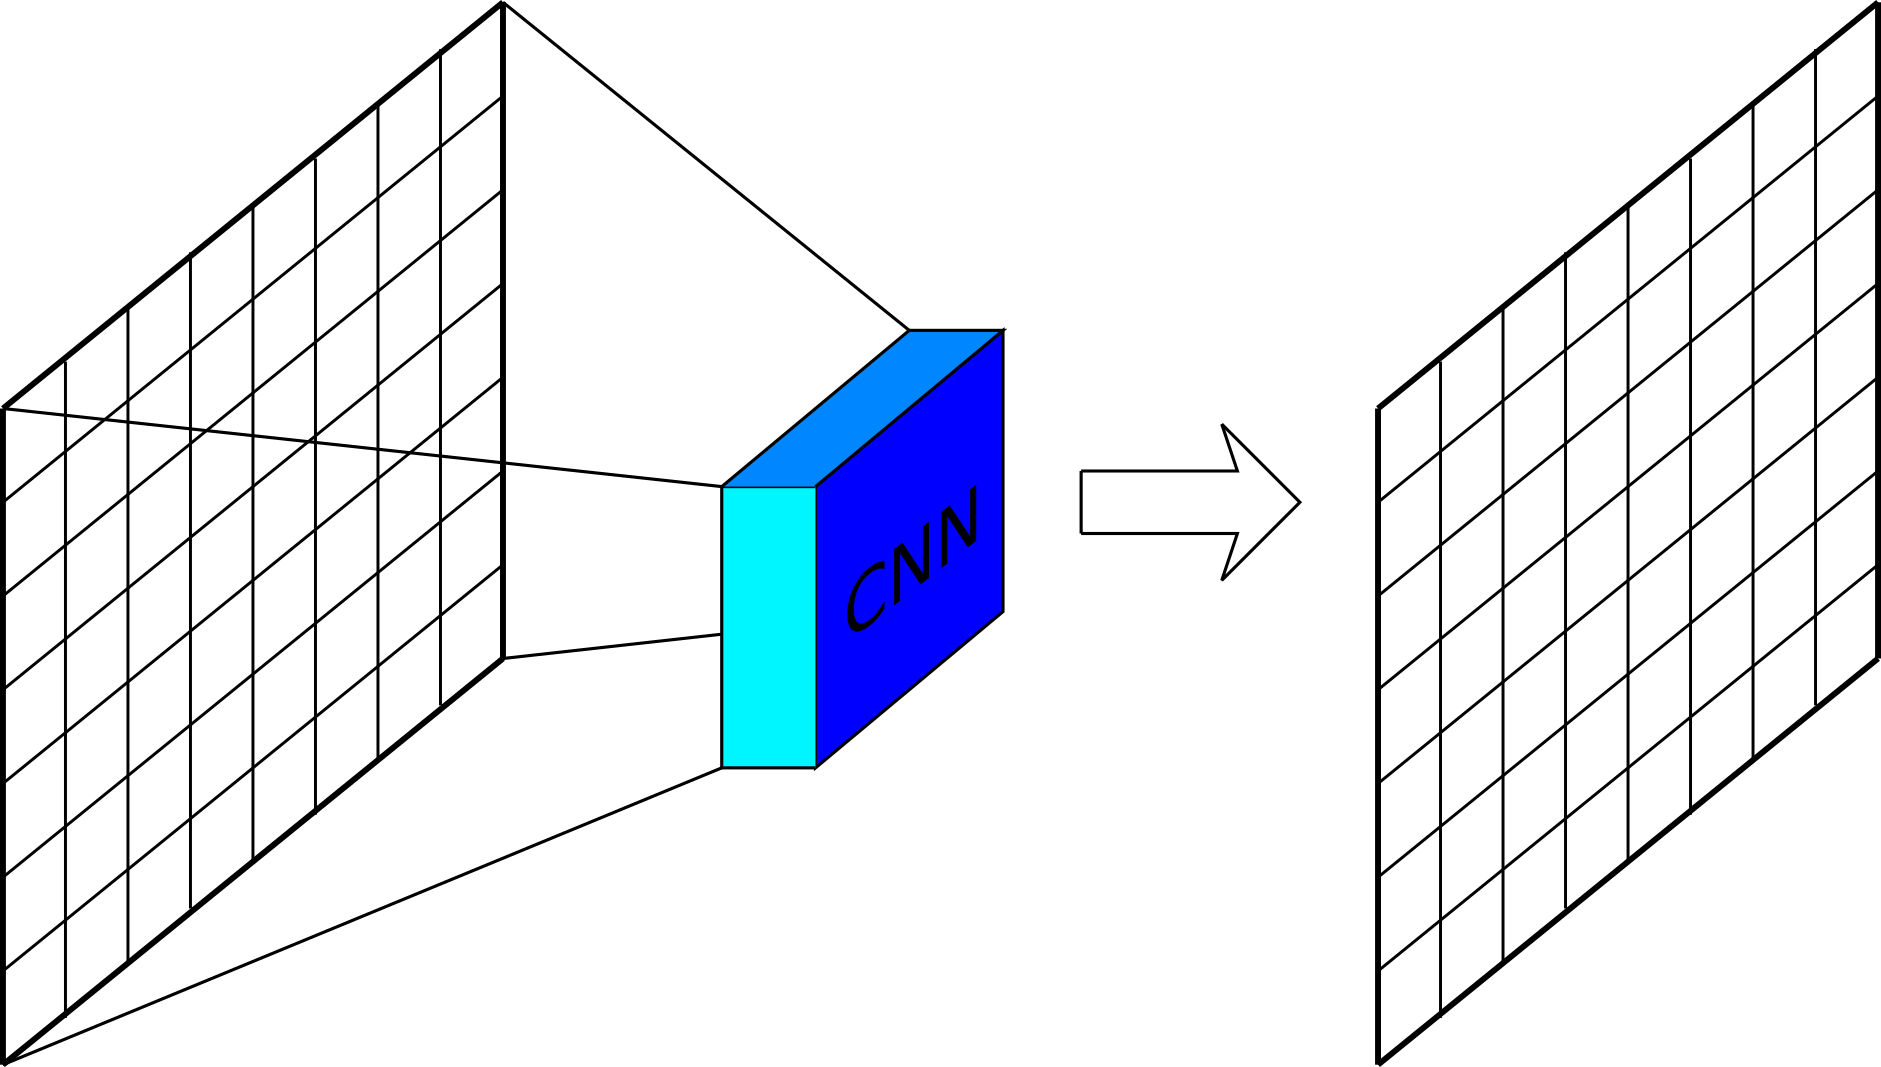
\includegraphics[width=0.40\textheight]{image_transf0.png}
      \end{figure}
  \end{itemize}

\end{frame}


%%%%%%%%%%%%%%%%%%%%%%%%%%%%%%%%%%%%%%%%%%%%%%%%%%
\frame{
  \frametitle{Image definition}

  \begin{block}{Definition}
 Here an image is a 2D array of size $p \times q$. Each array element belongs to $\R^d$. The dimension of the value space $d$, is often called the \alert{number of channels} of the image.

      The set of these images is $\mathcal{I}^d$.
  \end{block}

  \begin{block}{Examples}
    \begin{figure}
      \hfill
      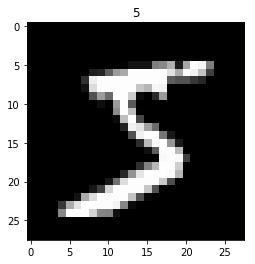
\includegraphics[width=2cm]{mnist_example_5}
      \hfill
      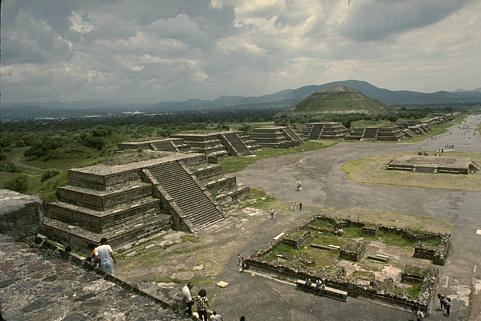
\includegraphics[width=4cm]{berkeley_db_33066.jpg}
      \caption{$28 \times 28$ grey level image $(d=1)$ from the MNIST data set, and $481 \times 321$ colour image $(d=3)$ from the Berkeley segmentation data set.}
    \end{figure}
  \end{block}


}


%%%%%%%%%%%%%%%%%%%%%%%%%%%%%%%%%%%%%%%%%%%%%%%%%%
\frame{
  \frametitle{Image-to-image translation}

  \begin{block}{Definition: image-to-image translation}
    An image-to-image operator is a function that transforms an image into another image of same size:
    \vspace{-1em}
    \begin{align*}
      F: \, \mathcal{I}^{d_1} & \longrightarrow \mathcal{I}^{d_2} \\
      I &  \longmapsto     J
    \end{align*}
    Note that the number of channels of input and output images can be different.
  \end{block}

      \begin{figure}
      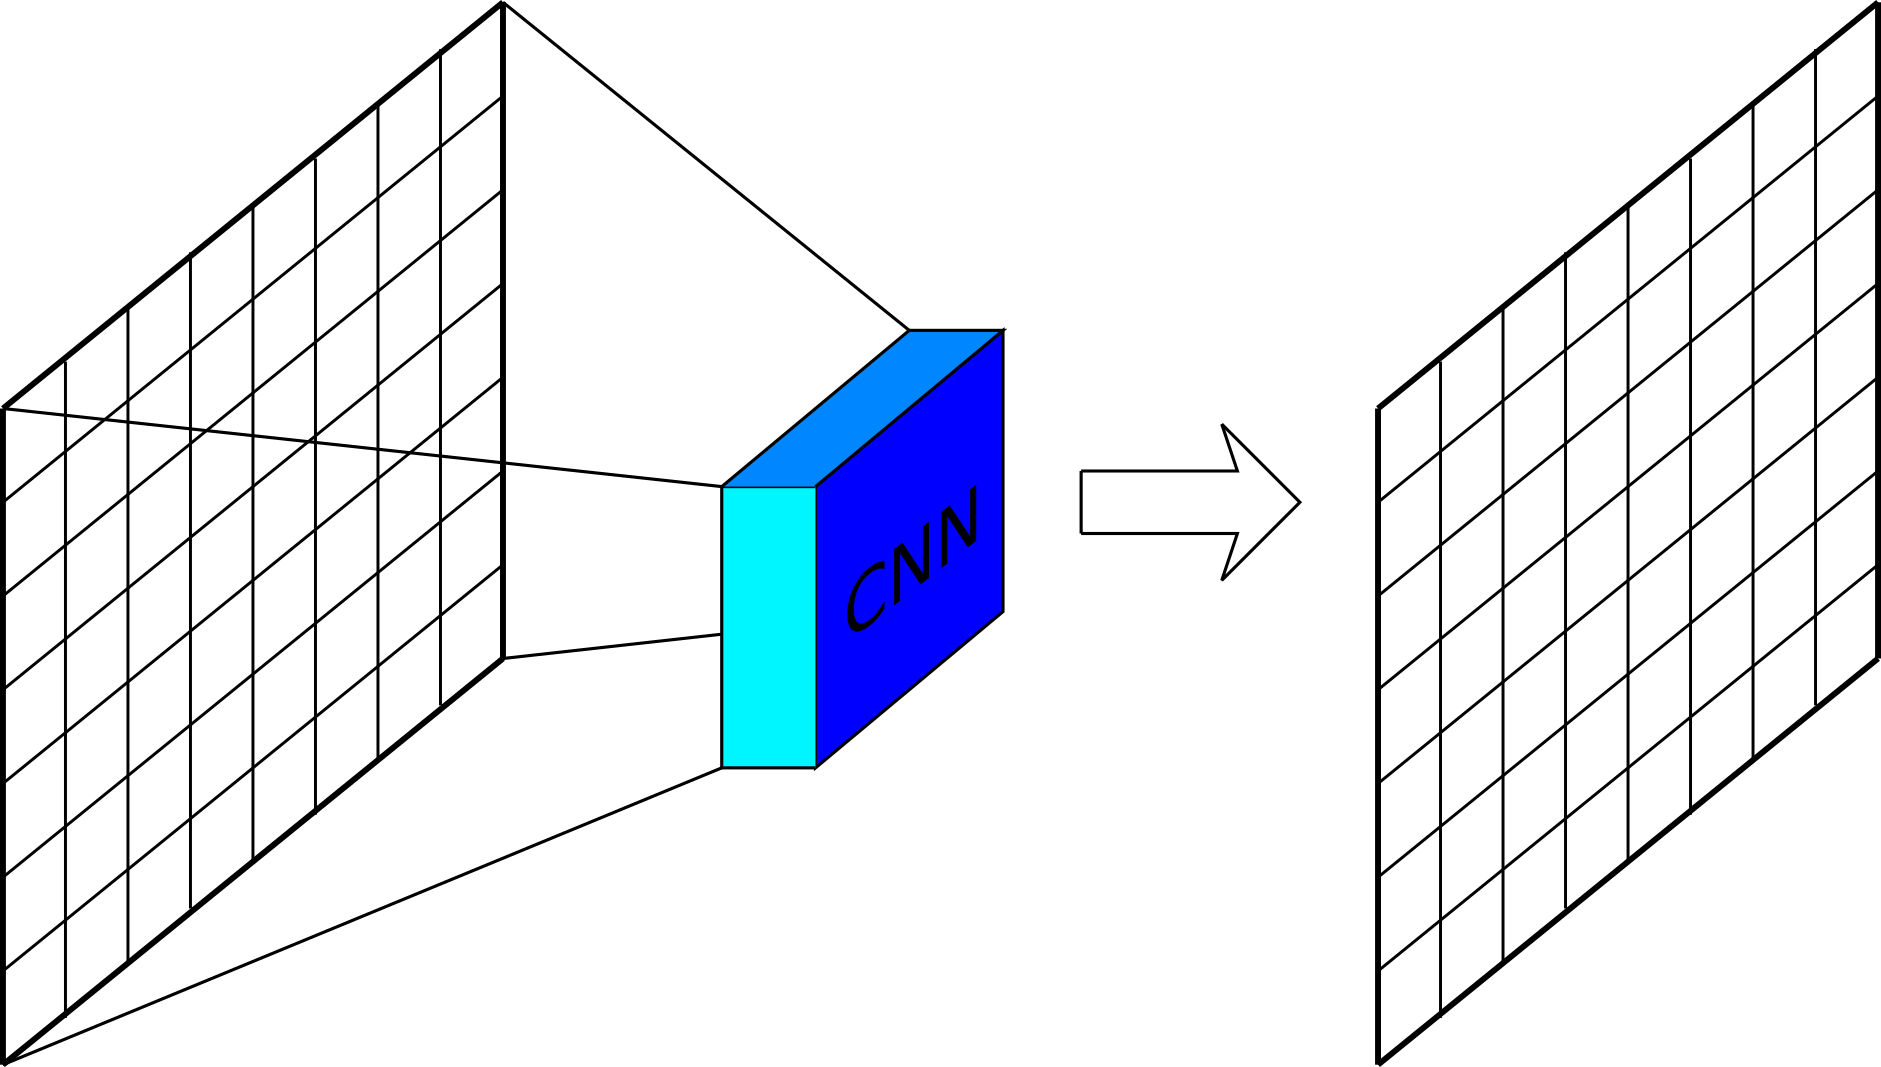
\includegraphics[width=0.40\textheight]{image_transf0.png}
      \end{figure}

}

%%%%%%%%%%%%%%%%%%%%%%%%%%%%%%%%%%%%%%%%%%%%%%%%%%
\frame{
  \frametitle{Examples}

  \begin{block}{Bulge / disk decomposition}
    \begin{figure}
      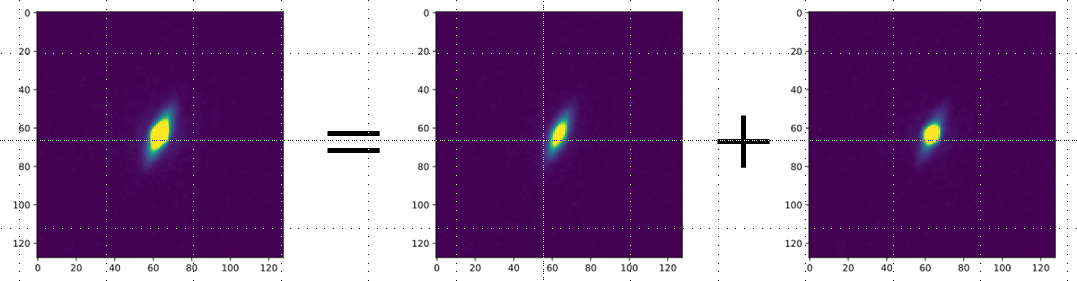
\includegraphics[width=8cm]{decomposition.png}\\
      \hfill {\tiny (Credits: Tuccillo, Huertas-Company, Velasco-Forero, Decencière)}
    \end{figure}
  \end{block}

  \pause

  \begin{block}{Deblurring network \cite{hradis_convolutional_2015}}
    \begin{figure}
      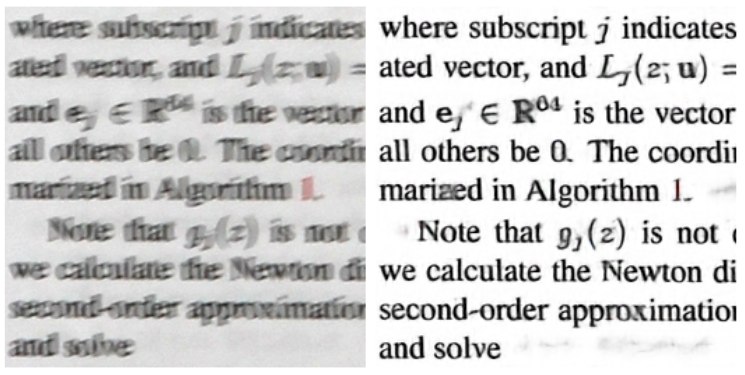
\includegraphics[width=4cm]{deblurring_hradis.png}
    \end{figure}
  \end{block}


}

%%%%%%%%%%%%%%%%%%%%%%%%%%%%%%%%%%%%%%%%%%%%%%%%%%
\frame{
  \frametitle{Pix2Pix}

    \begin{figure}
      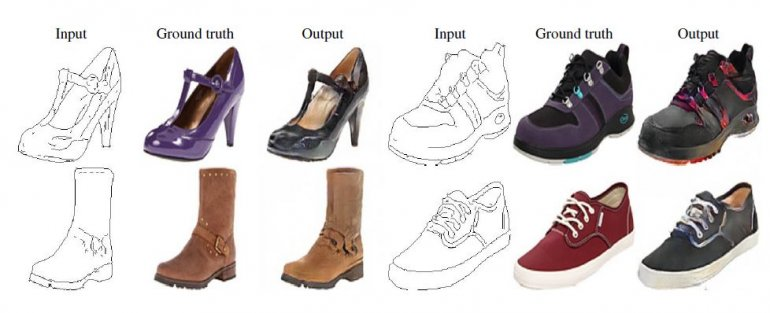
\includegraphics[width=\textwidth]{pix2pix}
      \source{https://neurohive.io/en/popular-networks/pix2pix-image-to-image-translation/}
    \end{figure}

}

%%%%%%%%%%%%%%%%%%%%%%%%%%%%%%%%%%%%%%%%%%%%%%%%%%
\frame{
  \frametitle{Counting cells}

    \begin{figure}
      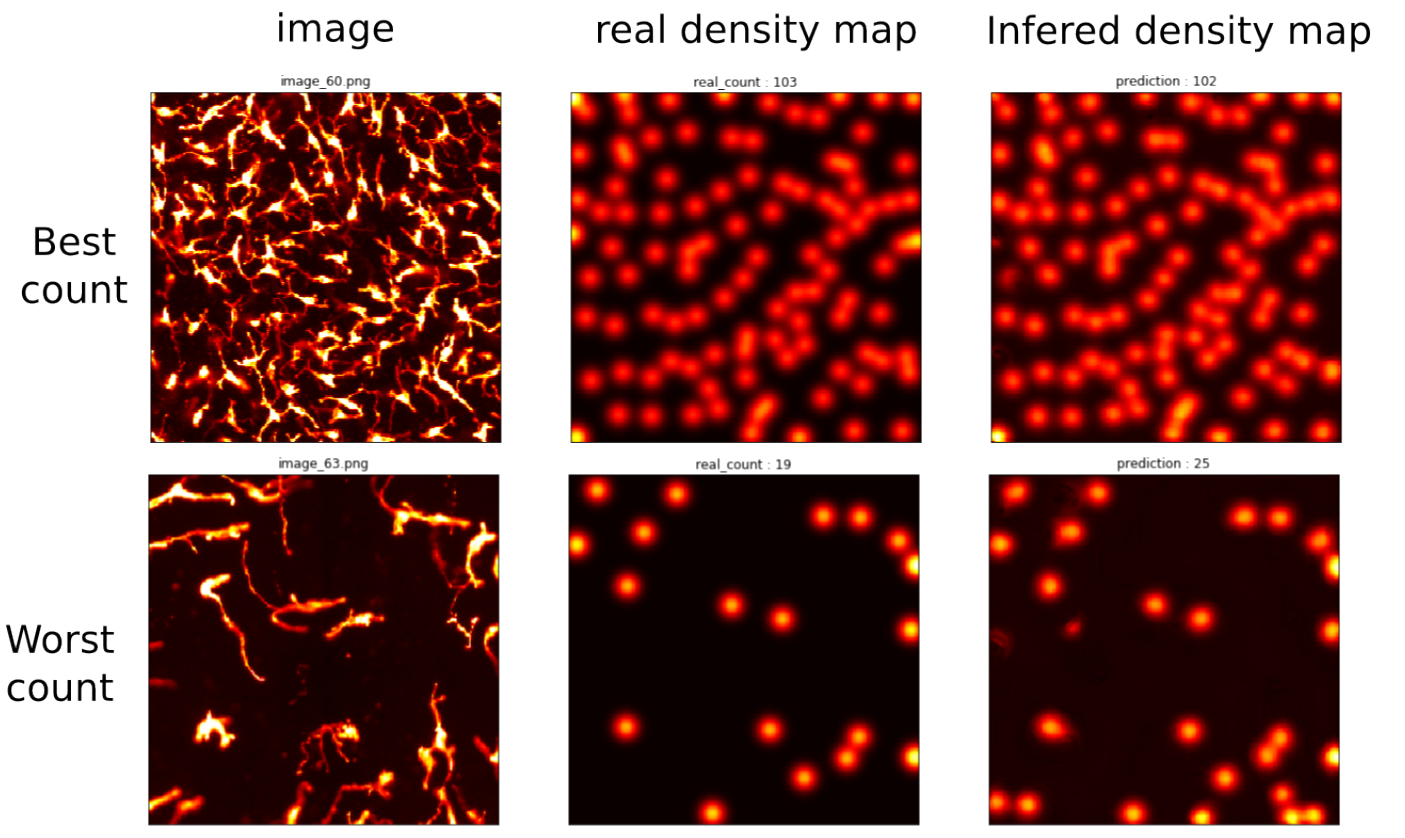
\includegraphics[width=\textwidth]{lazard}
      \source{Lazard, master report}
    \end{figure}

}

%%%%%%%%%%%%%%%%%%%%%%%%%%%%%%%%%%%%%%%%%%%%%%%%%%
\frame{
  \frametitle{Super resolution}

    \begin{figure}
      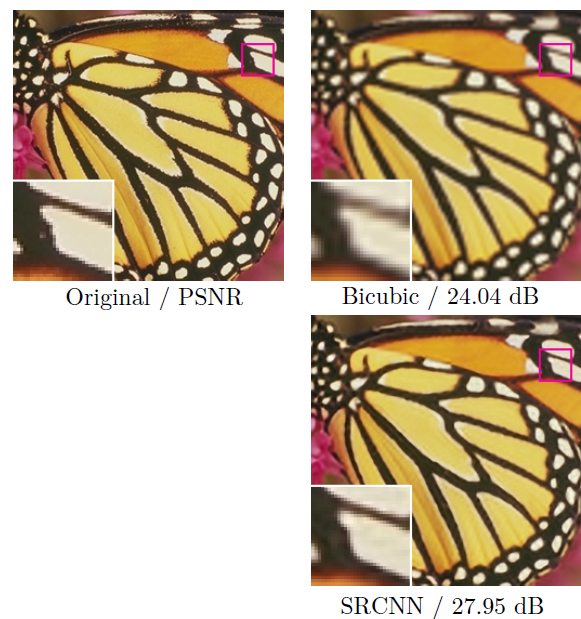
\includegraphics[height=0.8\textheight]{superres2}
      \source{http://mmlab.ie.cuhk.edu.hk/projects/SRCNN.html}
    \end{figure}

}

%%%%%%%%%%%%%%%%%%%%%%%%%%%%%%%%%%%%
\begin{frame}{Microscopy cross-modality prediction\cite{ounkomol_label-free_2018}}

  \begin{figure}[ht]
    \centering
    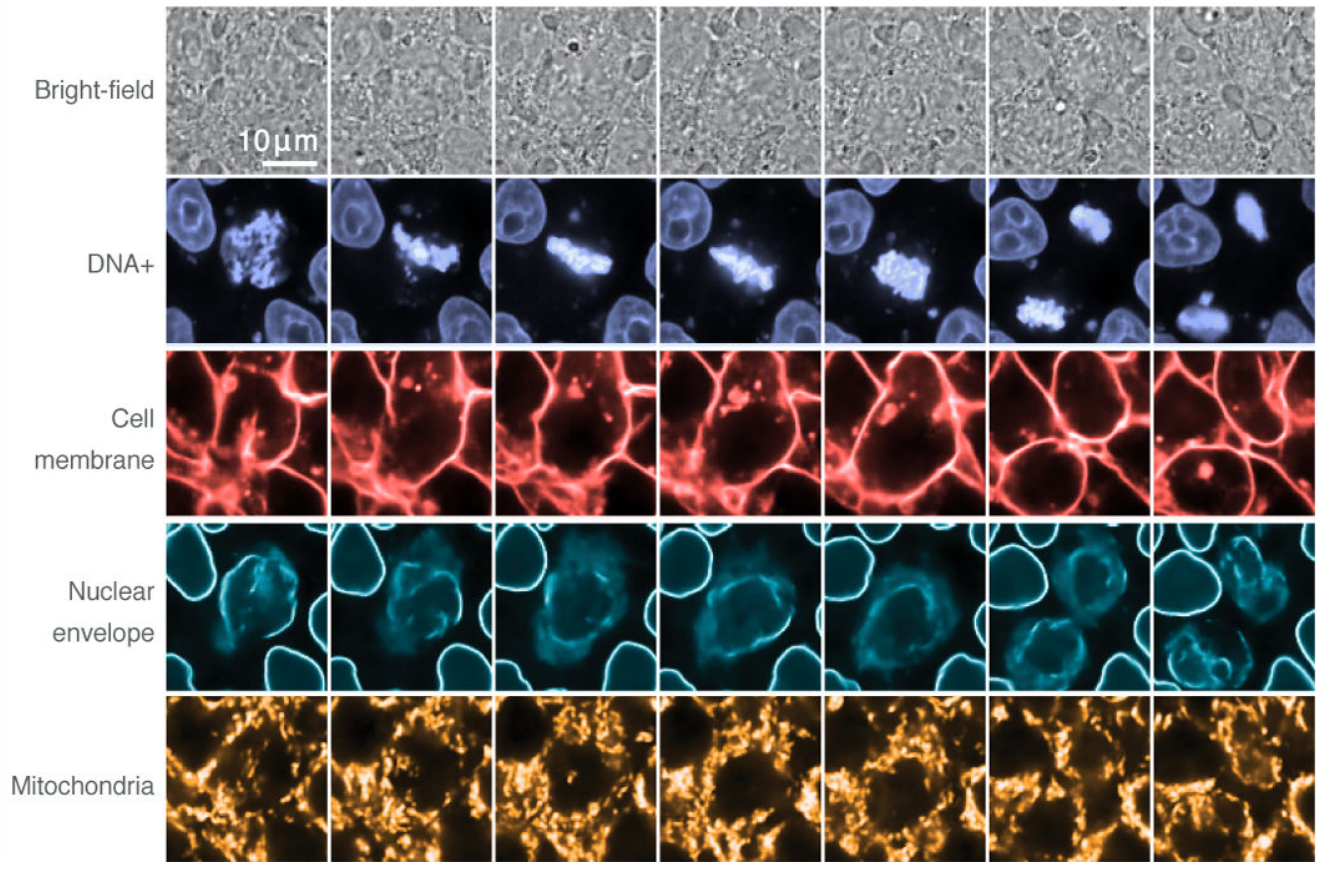
\includegraphics[width=\textwidth]{microscopy_modality_pred}
  \end{figure}



\end{frame}



%%%%%%%%%%%%%%%%%%%%%%%%%%%%%%%%%%%%%%%%%%%%%%%%%%
\frame{
  \frametitle{Image segmentation}

  \begin{itemize}

  \item Image segmentation is often an important step in an image processing work flow

  \item Image segmentation has been a very active deep learning research field

  \end{itemize}


  \begin{block}{Example}
    \begin{figure}
      \centering
      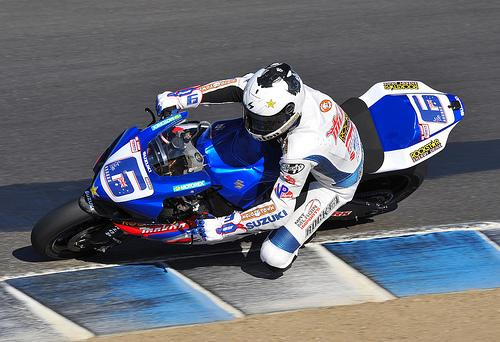
\includegraphics[height=2.5cm]{pascal_moto}
      \hspace{1em}
      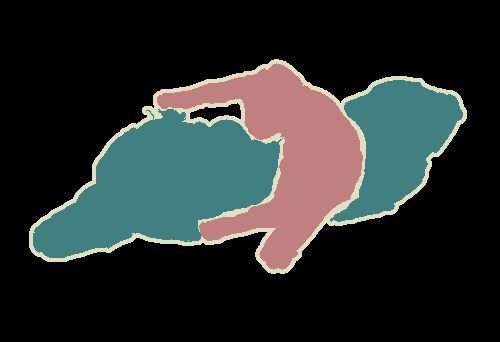
\includegraphics[height=2.5cm]{pascal_moto_seg}\\
      \source{Pascal VOC database}
    \end{figure}
  \end{block}

}

%%%%%%%%%%%%%%%%%%%%%%%%%%%%%%%%%%%%
\begin{frame}{Other applications}

  \begin{itemize}
  \item Image filtering
  \item High dynamic range
  \item Style modification
  \item Motion estimation
  \end{itemize}

  In the following, we will focus on image segmentation.

\end{frame}



%%%%%%%%%%%%%%%%%%%%%%%%%%%%%%%%%%%%
\section{From classification to image-to-image translation}




%%%%%%%%%%%%%%%%%%%%%%%%%%%%%%%%%%%%
\begin{frame}{VGG16: an example network for image classification}

  \begin{center}
    \begin{figure}
      \centering
      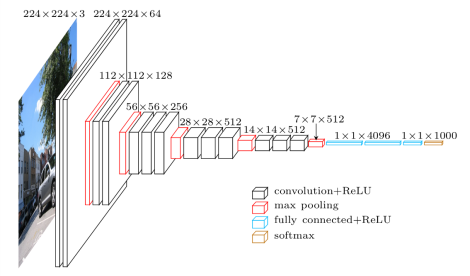
\includegraphics[width=0.65\textwidth]{vgg16.png}
      \source{VGG16 (From https://www.cs.toronto.edu/~frossard/post/vgg16/)}
    \end{figure}
  \end{center}


\end{frame}



%%%%%%%%%%%%%%%%%%%%%%%%%%%%%%%%%%%%
\begin{frame}{From classification nets to image-to-image nets}

      \begin{figure}
      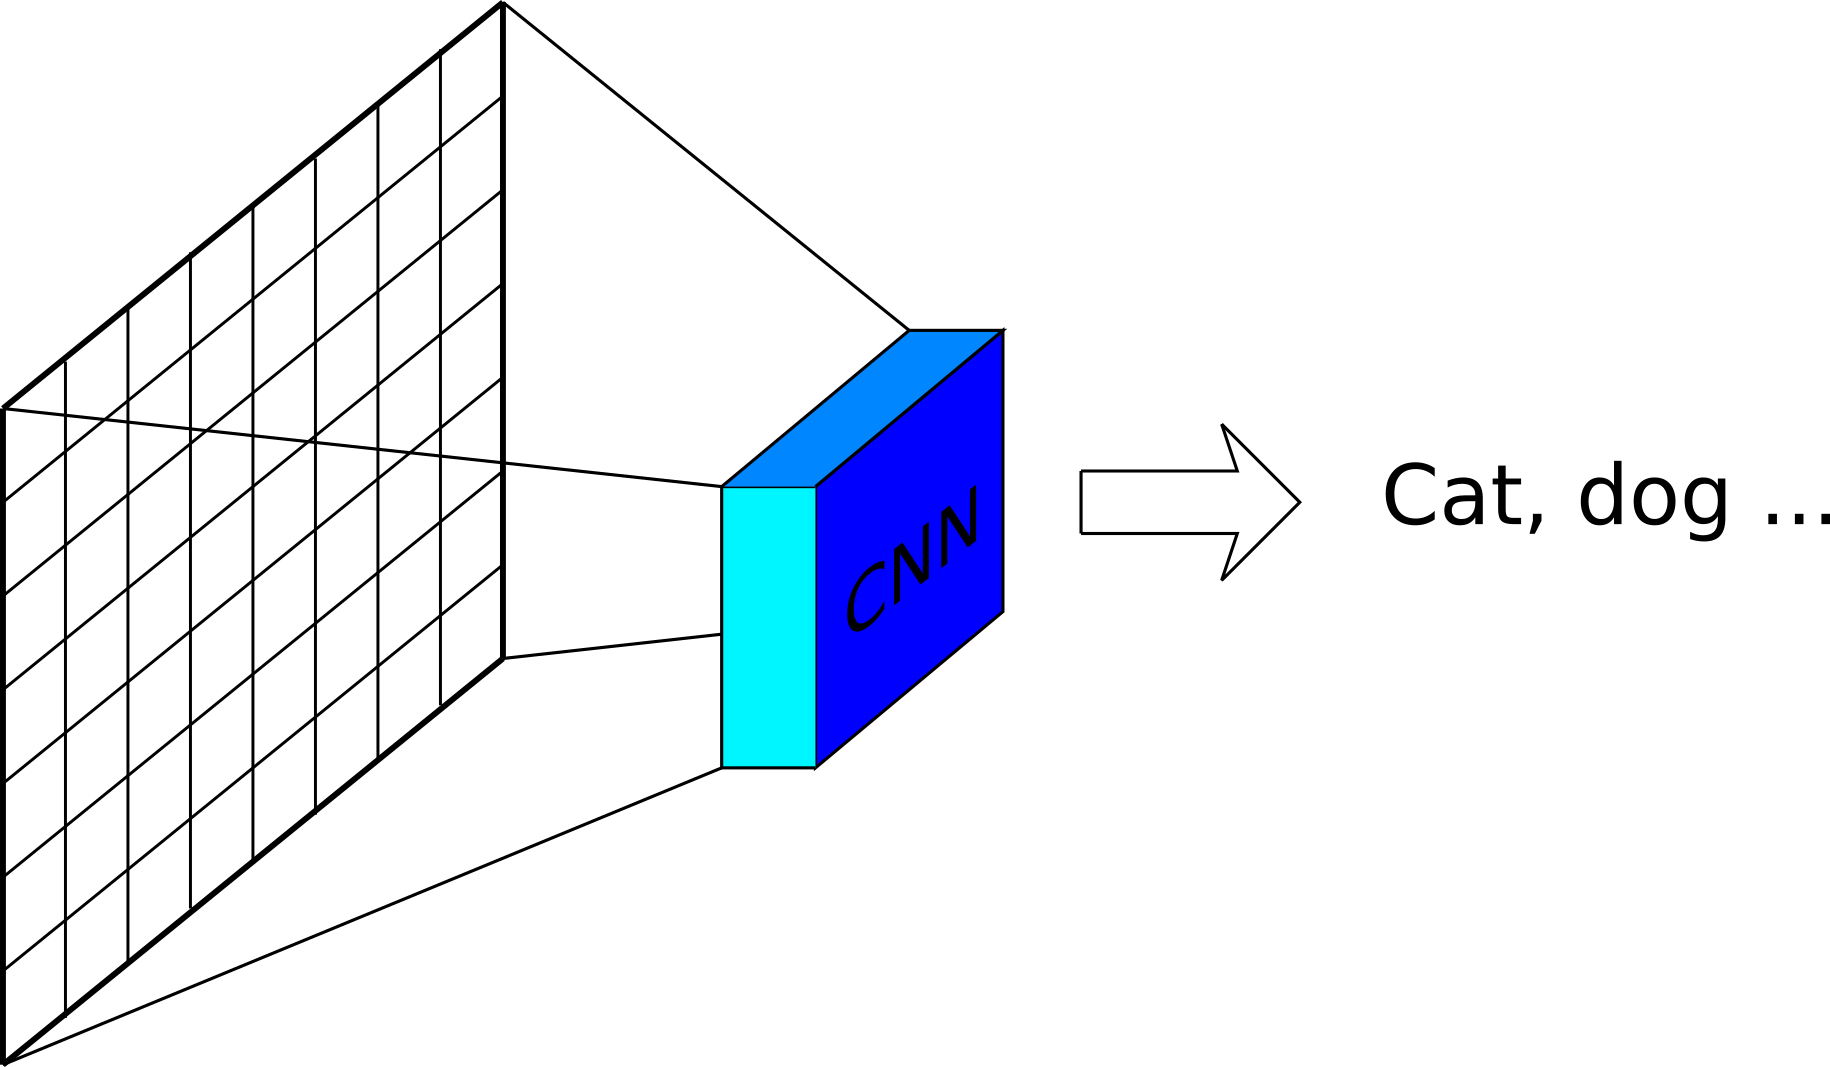
\includegraphics[width=0.5\textwidth]{image_classif.png}
      \end{figure}

      \pause

      \begin{figure}
      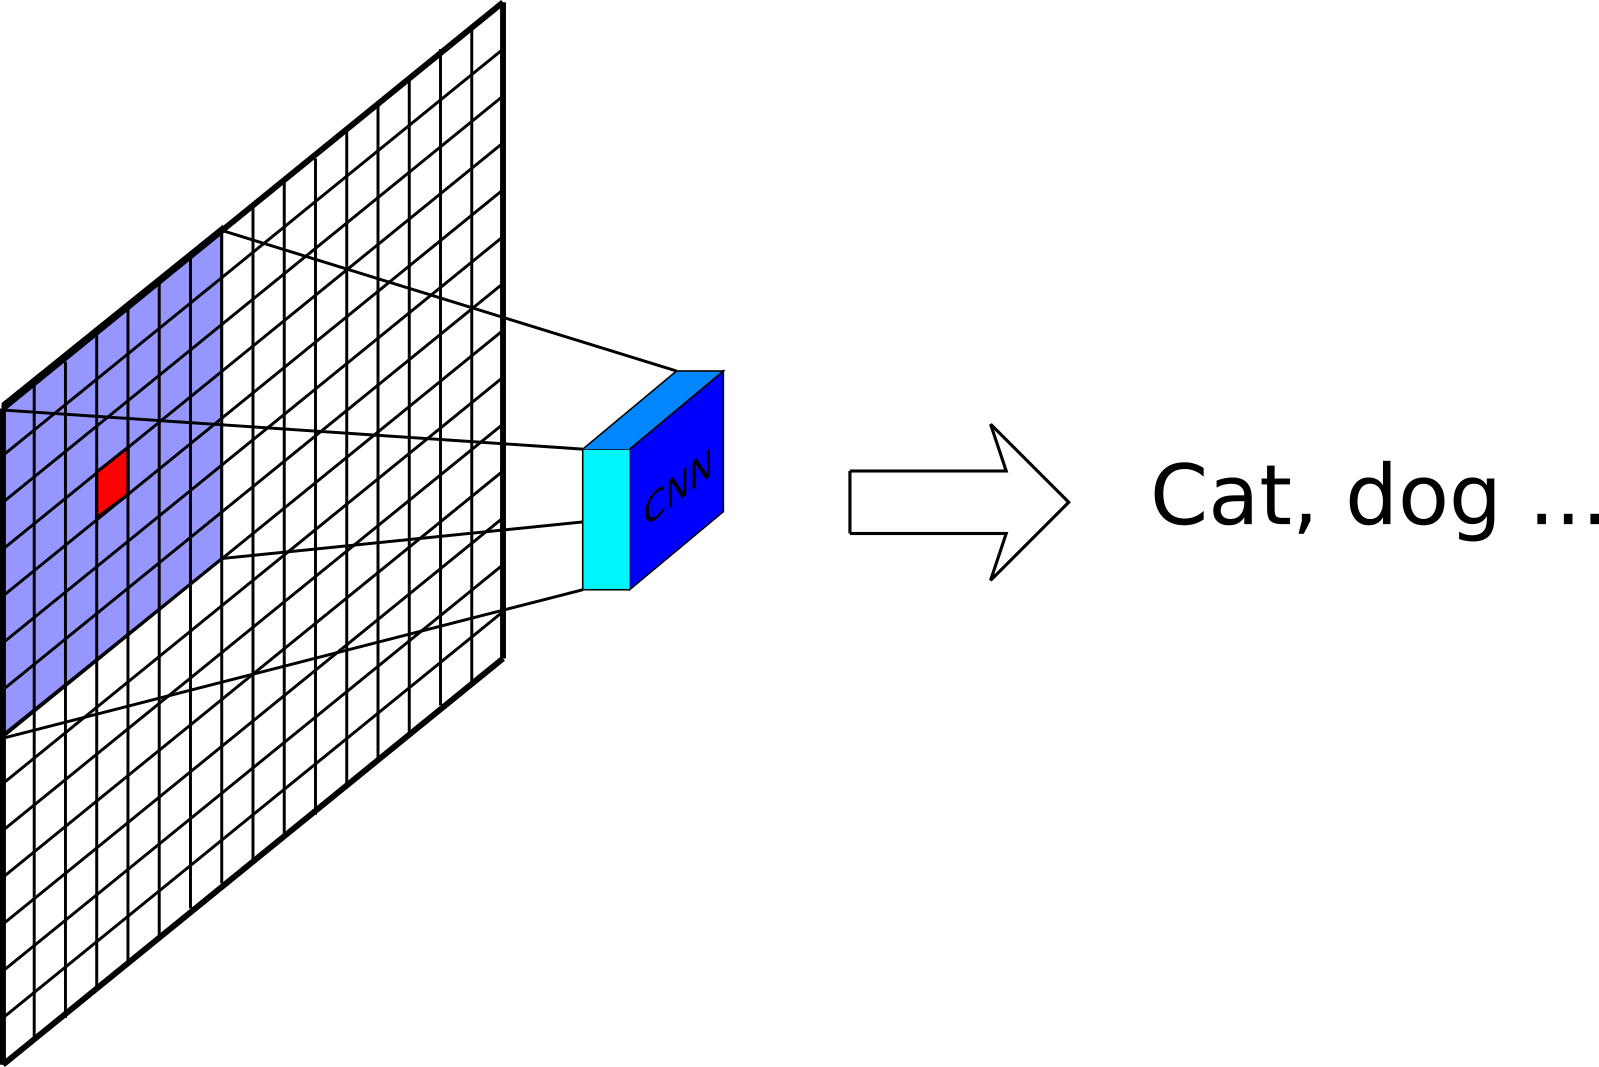
\includegraphics[width=0.5\textwidth]{image_transf.png}
      \end{figure}


\end{frame}


%%%%%%%%%%%%%%%%%%%%%%%%%%%%%%%%%%%%
\begin{frame}{From classification nets to image-to-image nets}

      \begin{figure}
      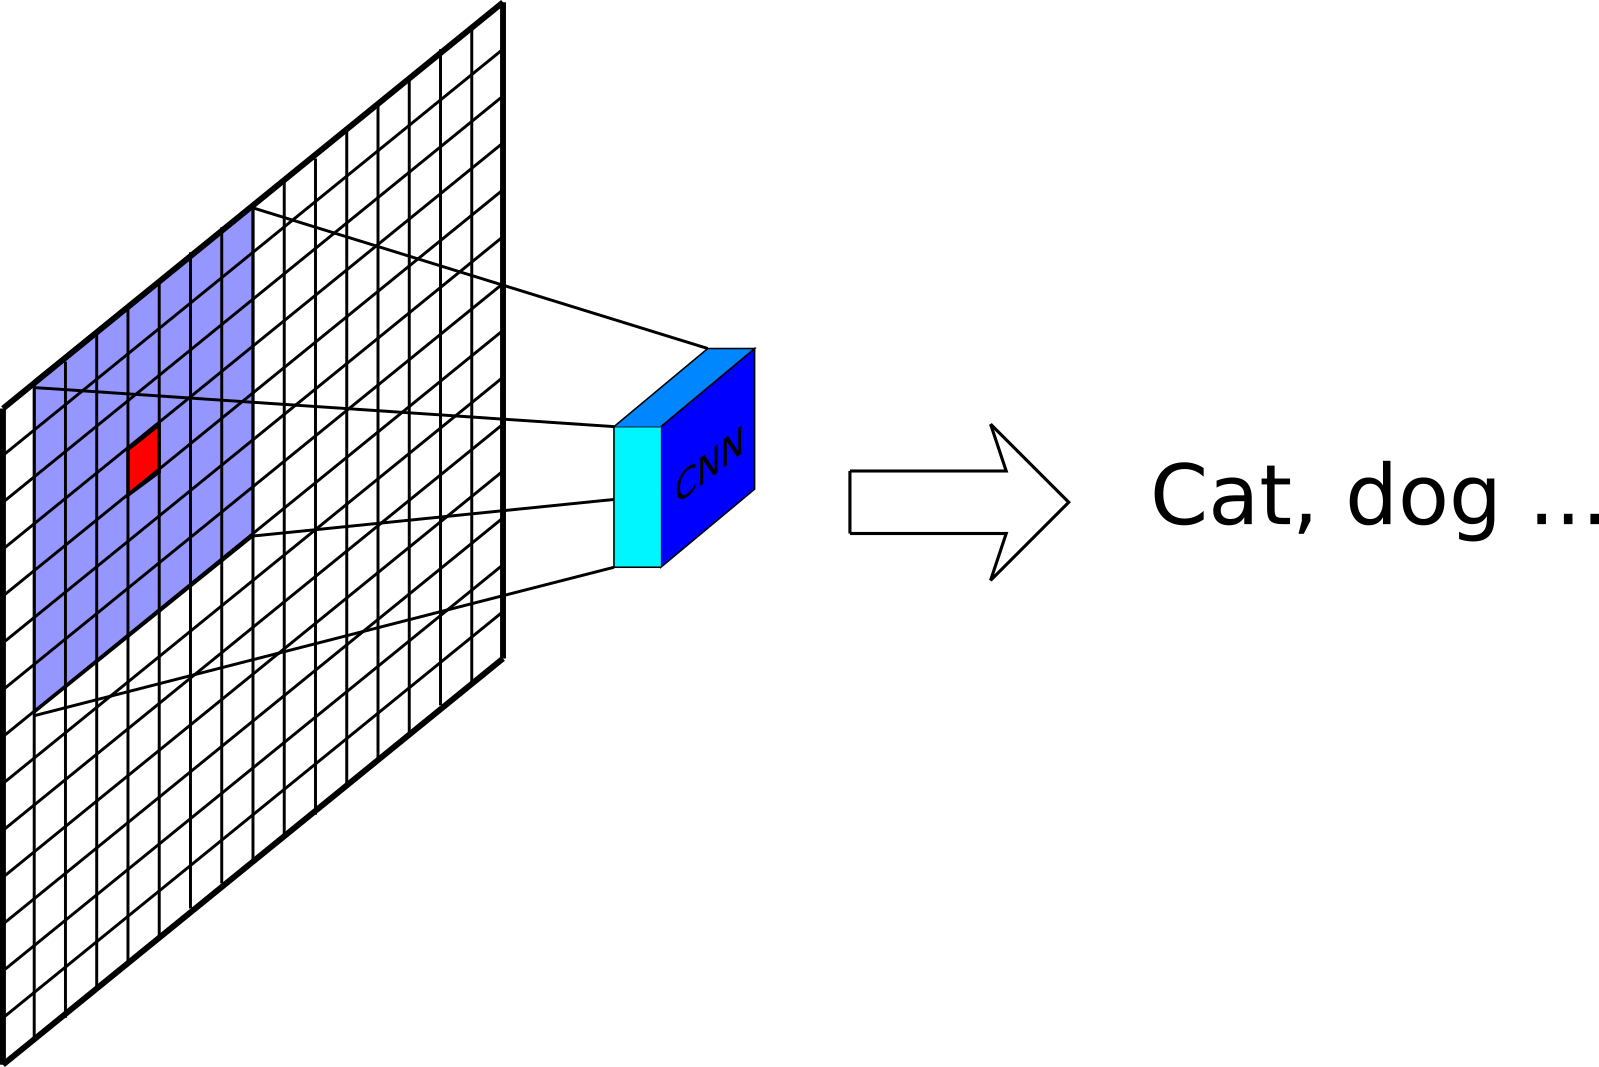
\includegraphics[width=0.5\textwidth]{image_transf1.png}
      \end{figure}

      \pause

      \begin{figure}
      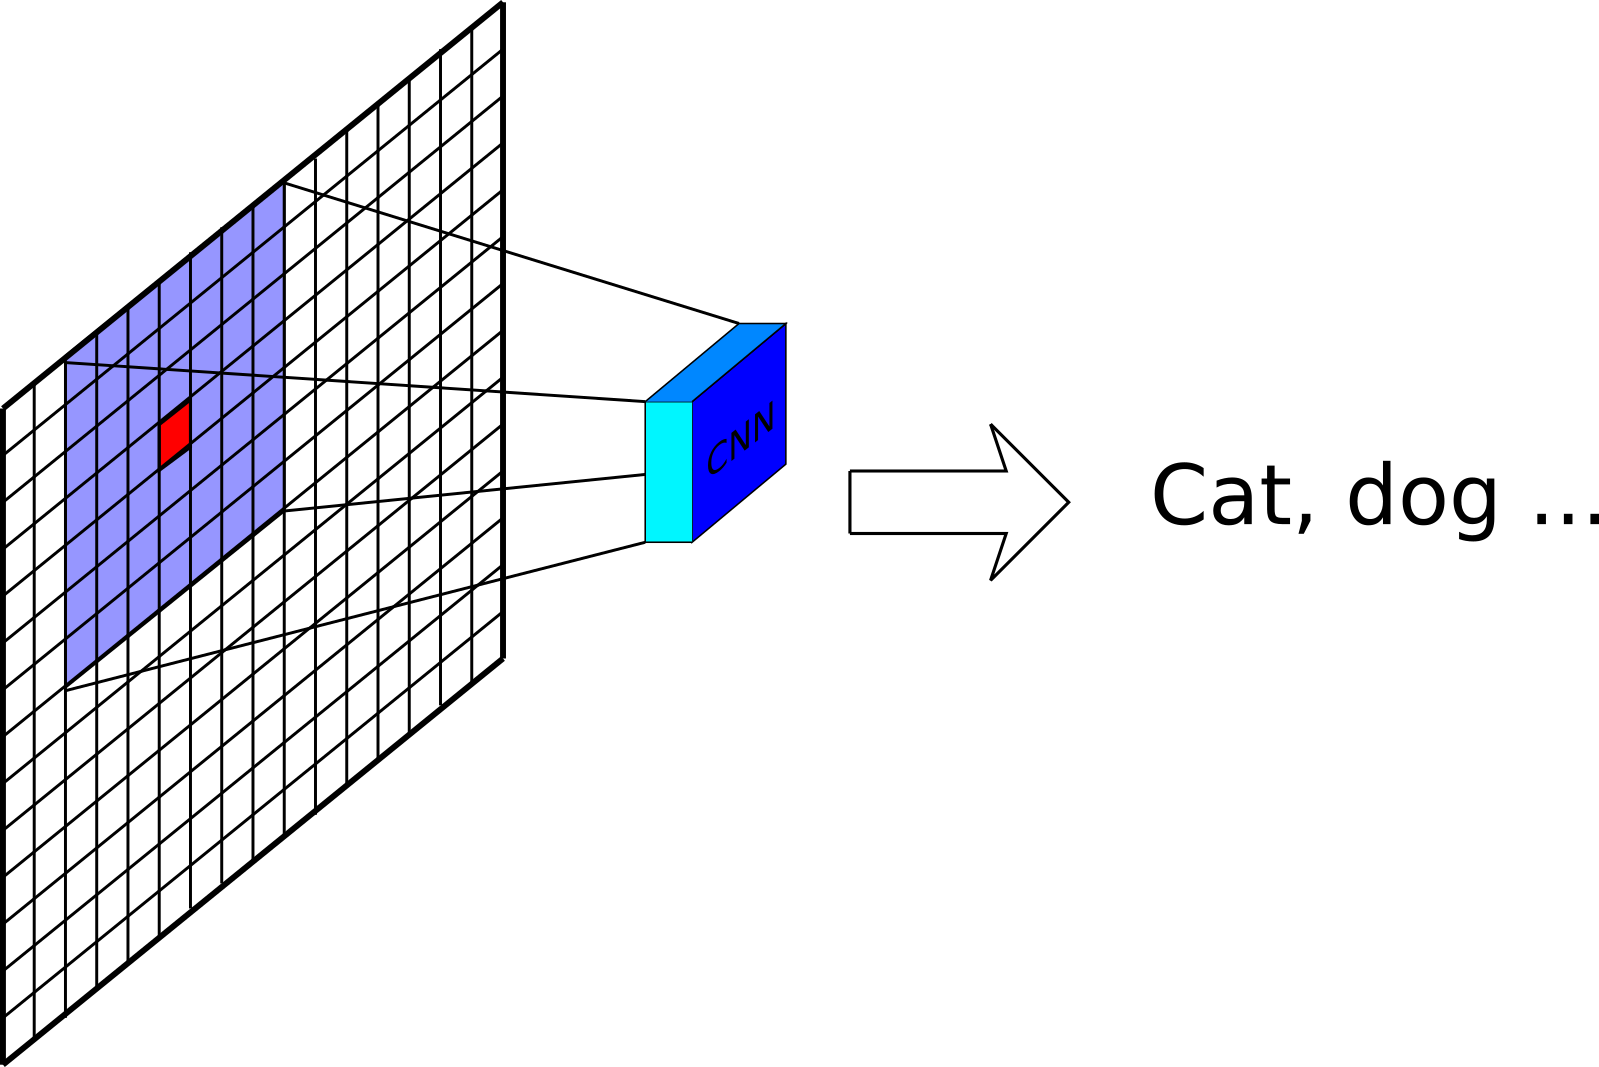
\includegraphics[width=0.5\textwidth]{image_transf2.png}
      \end{figure}

\end{frame}

%%%%%%%%%%%%%%%%%%%%%%%%%%%%%%%%%%%%
\begin{frame}{From classification nets to image-to-image nets}

      \begin{figure}
      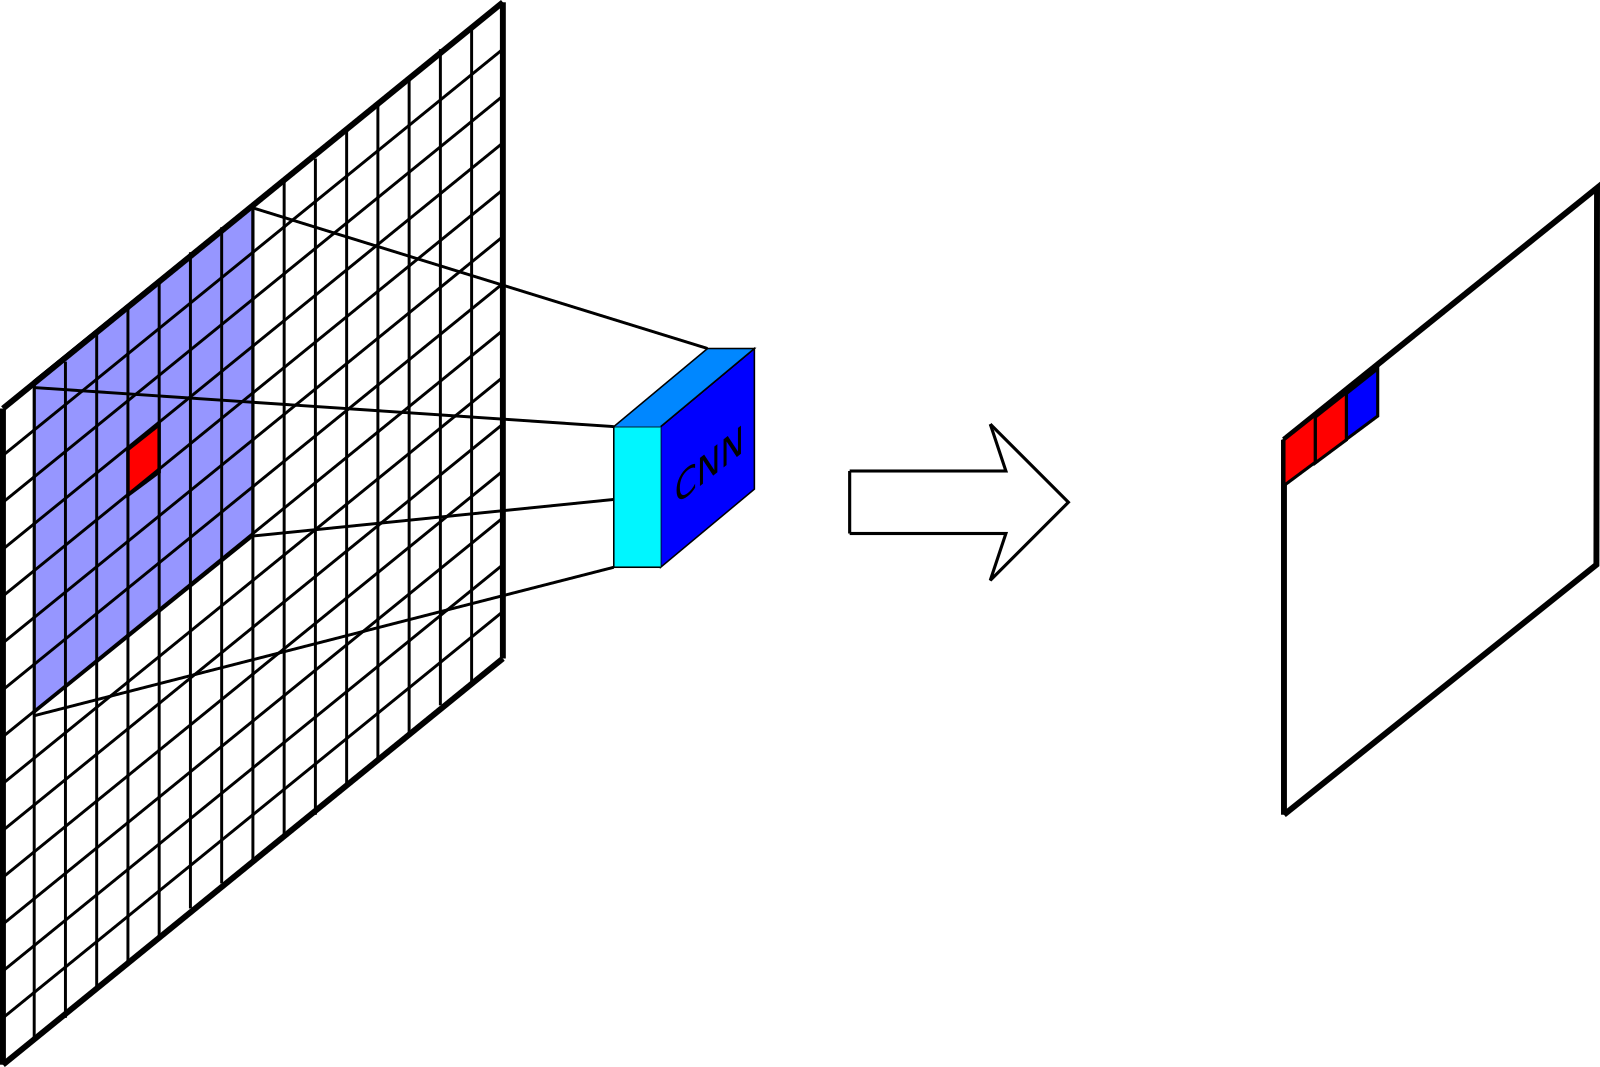
\includegraphics[width=0.5\textwidth]{image_transf_fin.png}
      \end{figure}

      The neuron membrane segmentation challenge winner~\cite{ciresan_deep_2012} used this strategy. It is inefficient.



\end{frame}


%%%%%%%%%%%%%%%%%%%%%%%%%%%%%%%%%%%%%%%%%%%%%%%%%%
\frame{
  \frametitle{The simplest image-to-image architecture}

  \begin{block}{Example: plain CNN \cite{pang_cell_2010}}
    \begin{figure}
      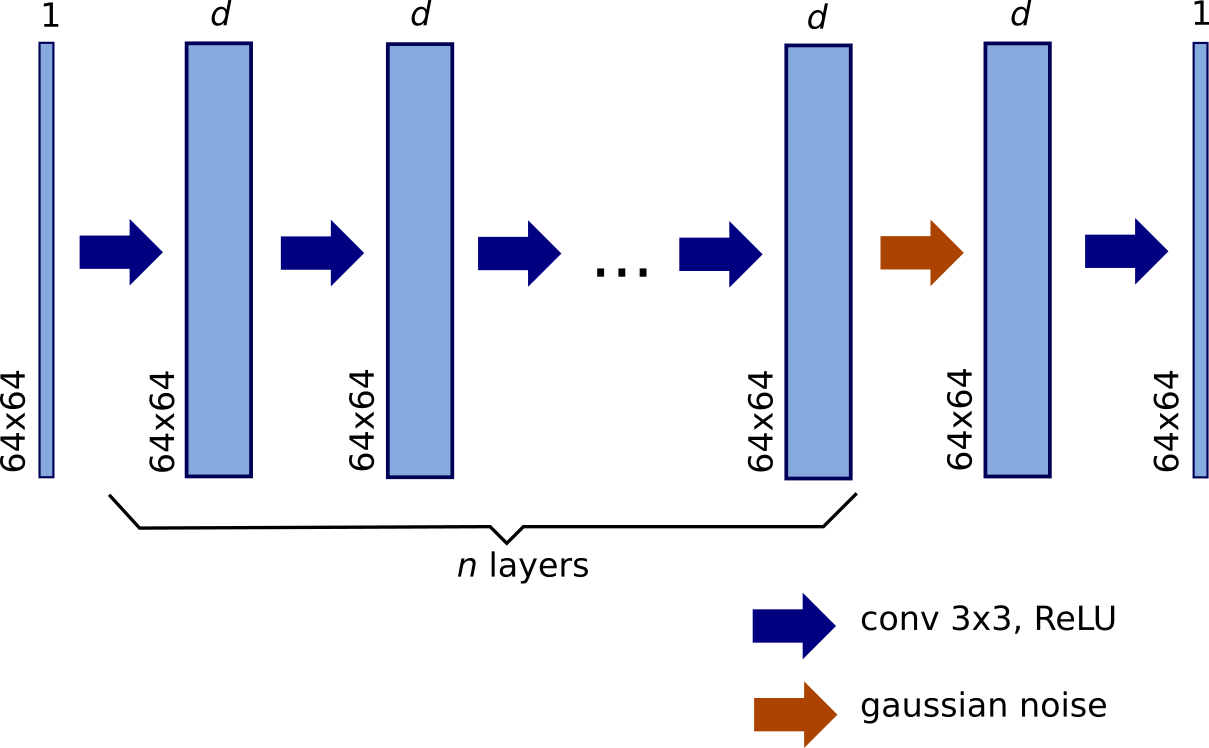
\includegraphics[width=\textwidth]{plain_convnet.png}
    \end{figure}
  \end{block}

}

%%%%%%%%%%%%%%%%%%%%%%%%%%%%%%%%%%%%
\begin{frame}<beamer>{Going back to the original image size}

    \begin{figure}
      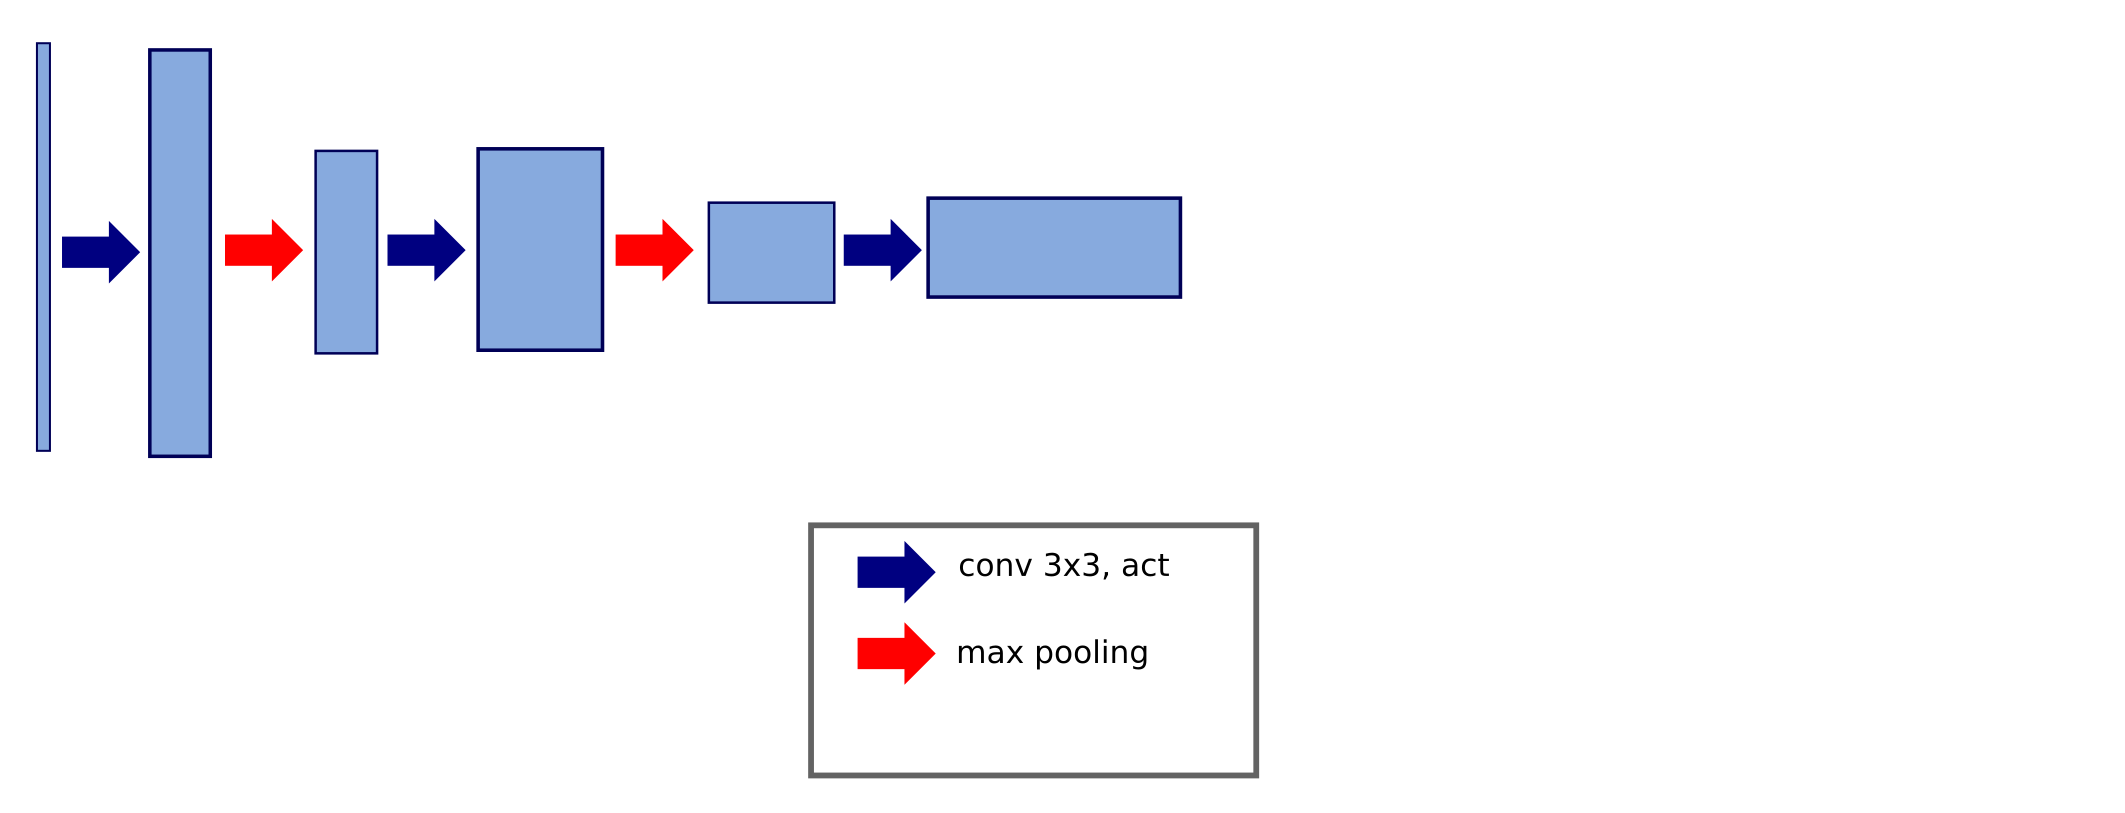
\includegraphics[width=\textwidth]{going_back1.png}
    \end{figure}

\end{frame}


%%%%%%%%%%%%%%%%%%%%%%%%%%%%%%%%%%%%
\begin{frame}<beamer>{Going back to the original image size}

    \begin{figure}
      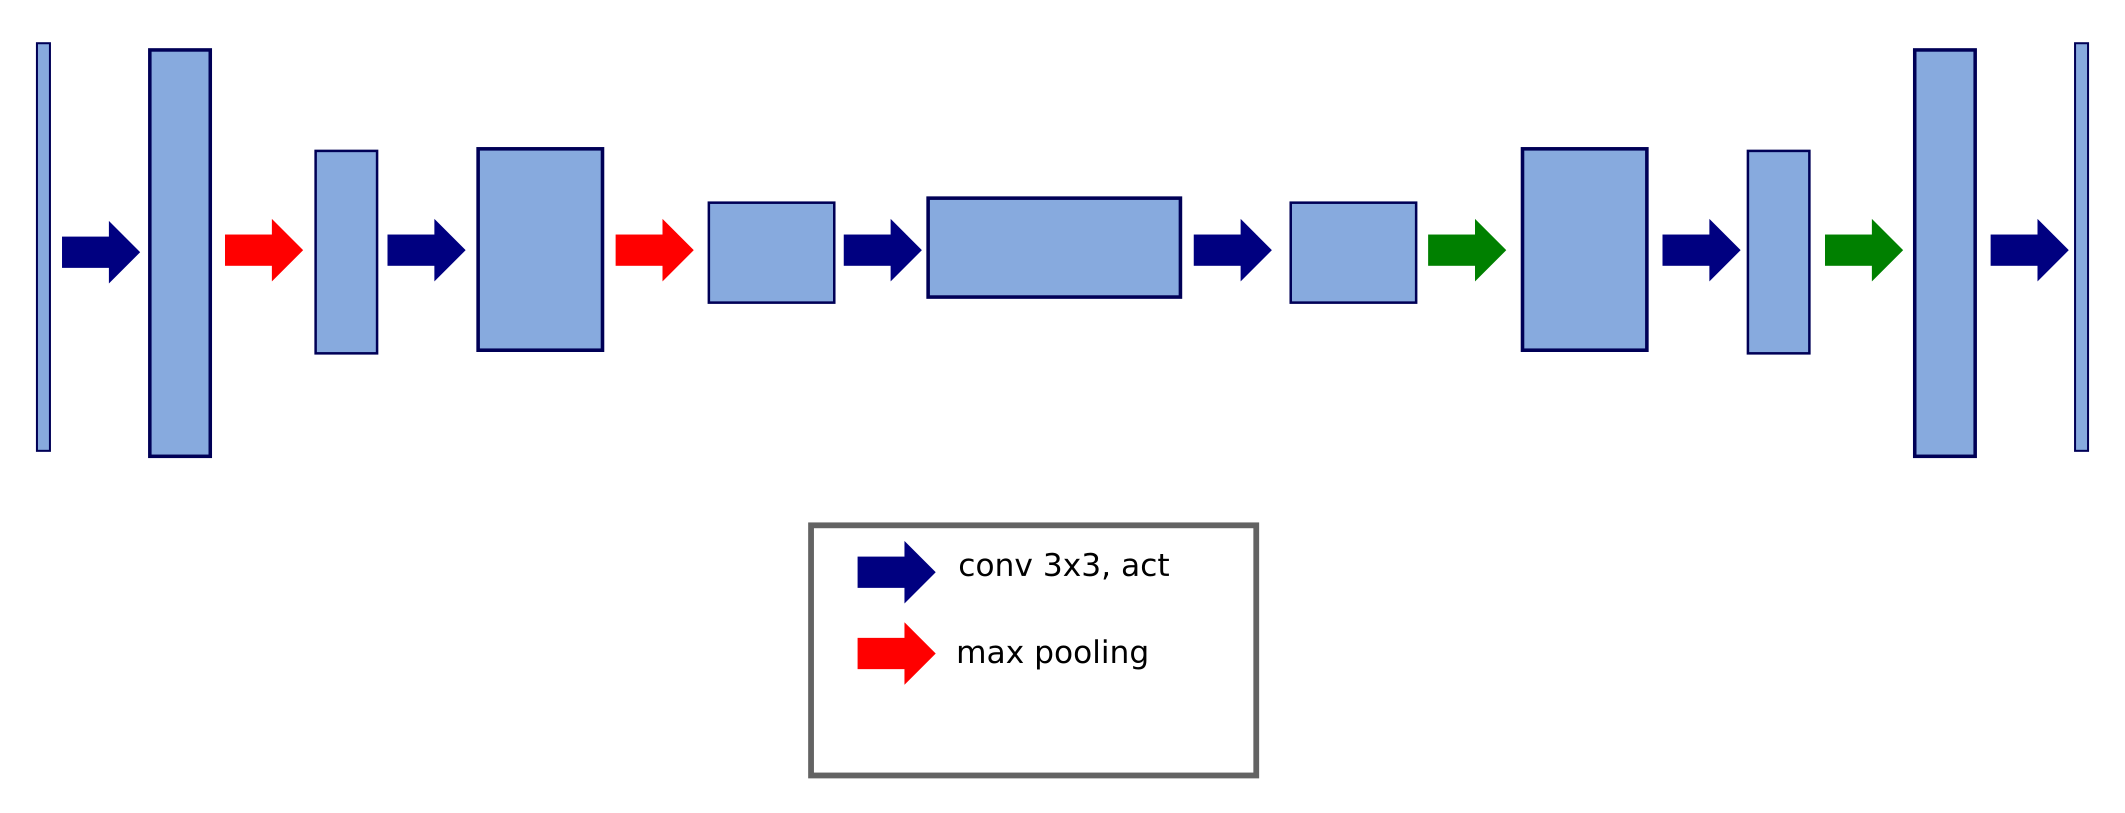
\includegraphics[width=\textwidth]{going_back2.png}
    \end{figure}

\end{frame}


%%%%%%%%%%%%%%%%%%%%%%%%%%%%%%%%%%%%
\begin{frame}{Going back to the original image size}

    \begin{figure}
      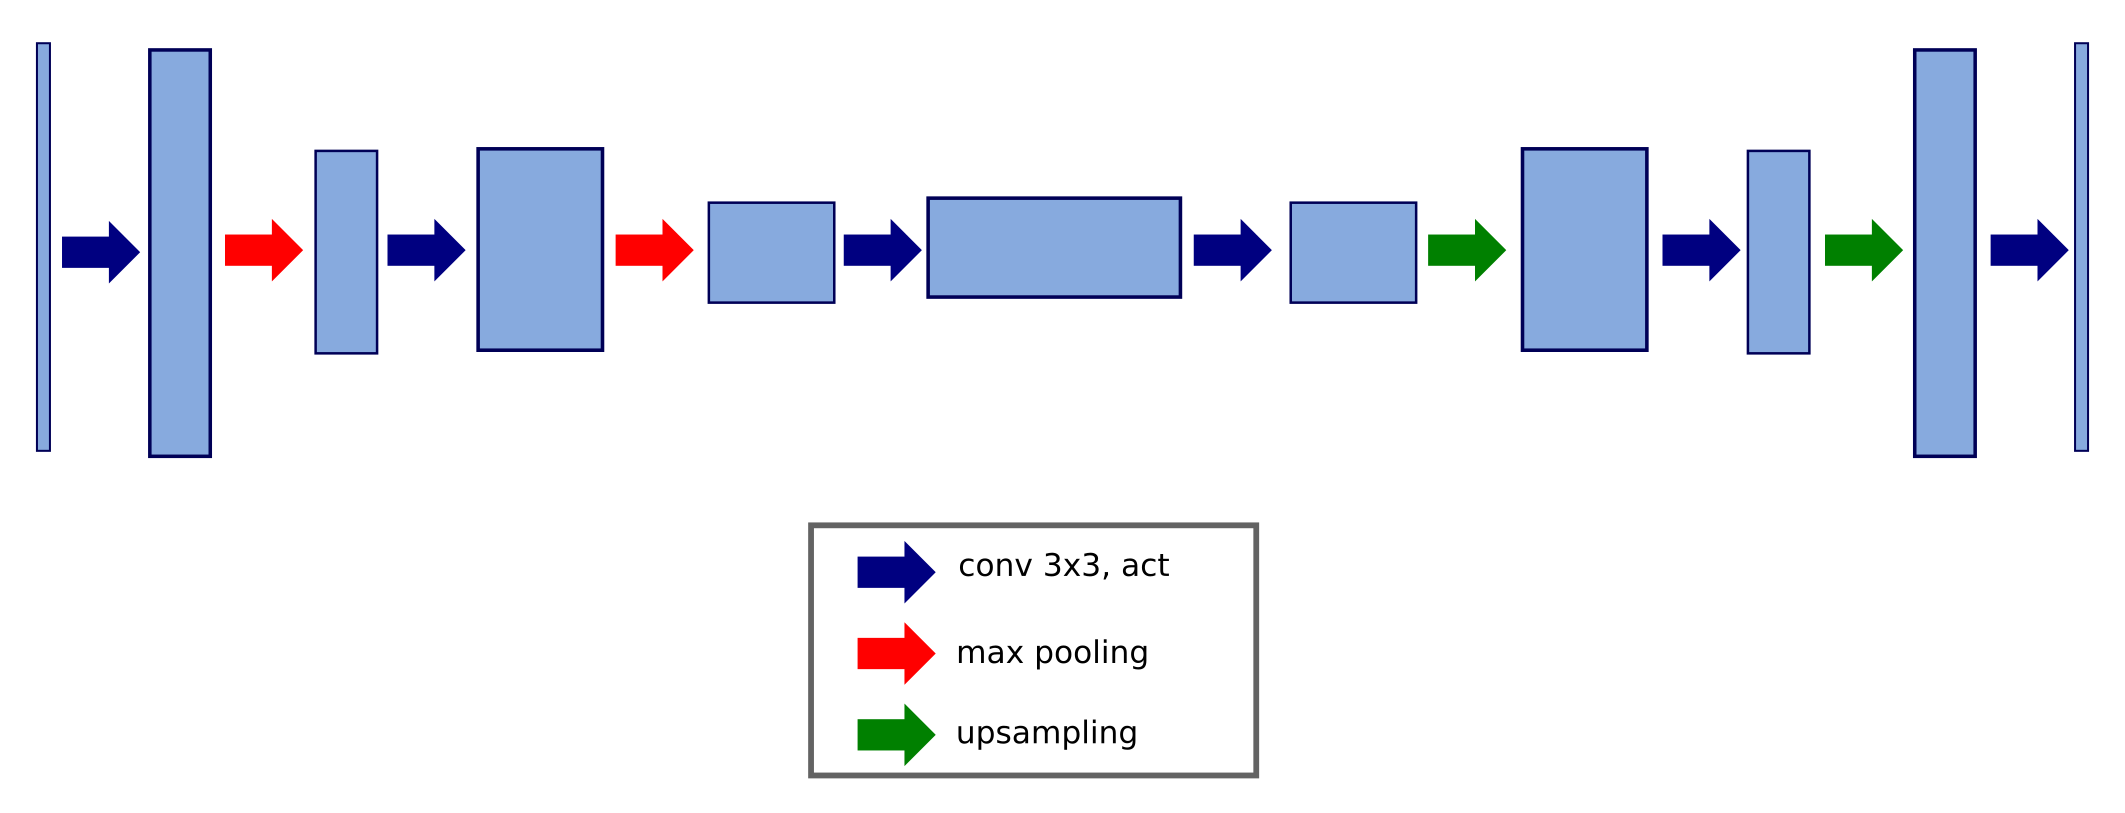
\includegraphics[width=\textwidth]{going_back.png}
    \end{figure}

\end{frame}


%%%%%%%%%%%%%%%%%%%%%%%%%%%%%%%%%%%%
\begin{frame}{Upsampling techniques}


\begin{itemize}
\item Replication
\item Pooling index memorization
\item Transposed convolution
\end{itemize}

\end{frame}

%%%%%%%%%%%%%%%%%%%%%%%%%%%%%%%%%%%%
\begin{frame}{Upsampling through replication}

  \begin{figure}
      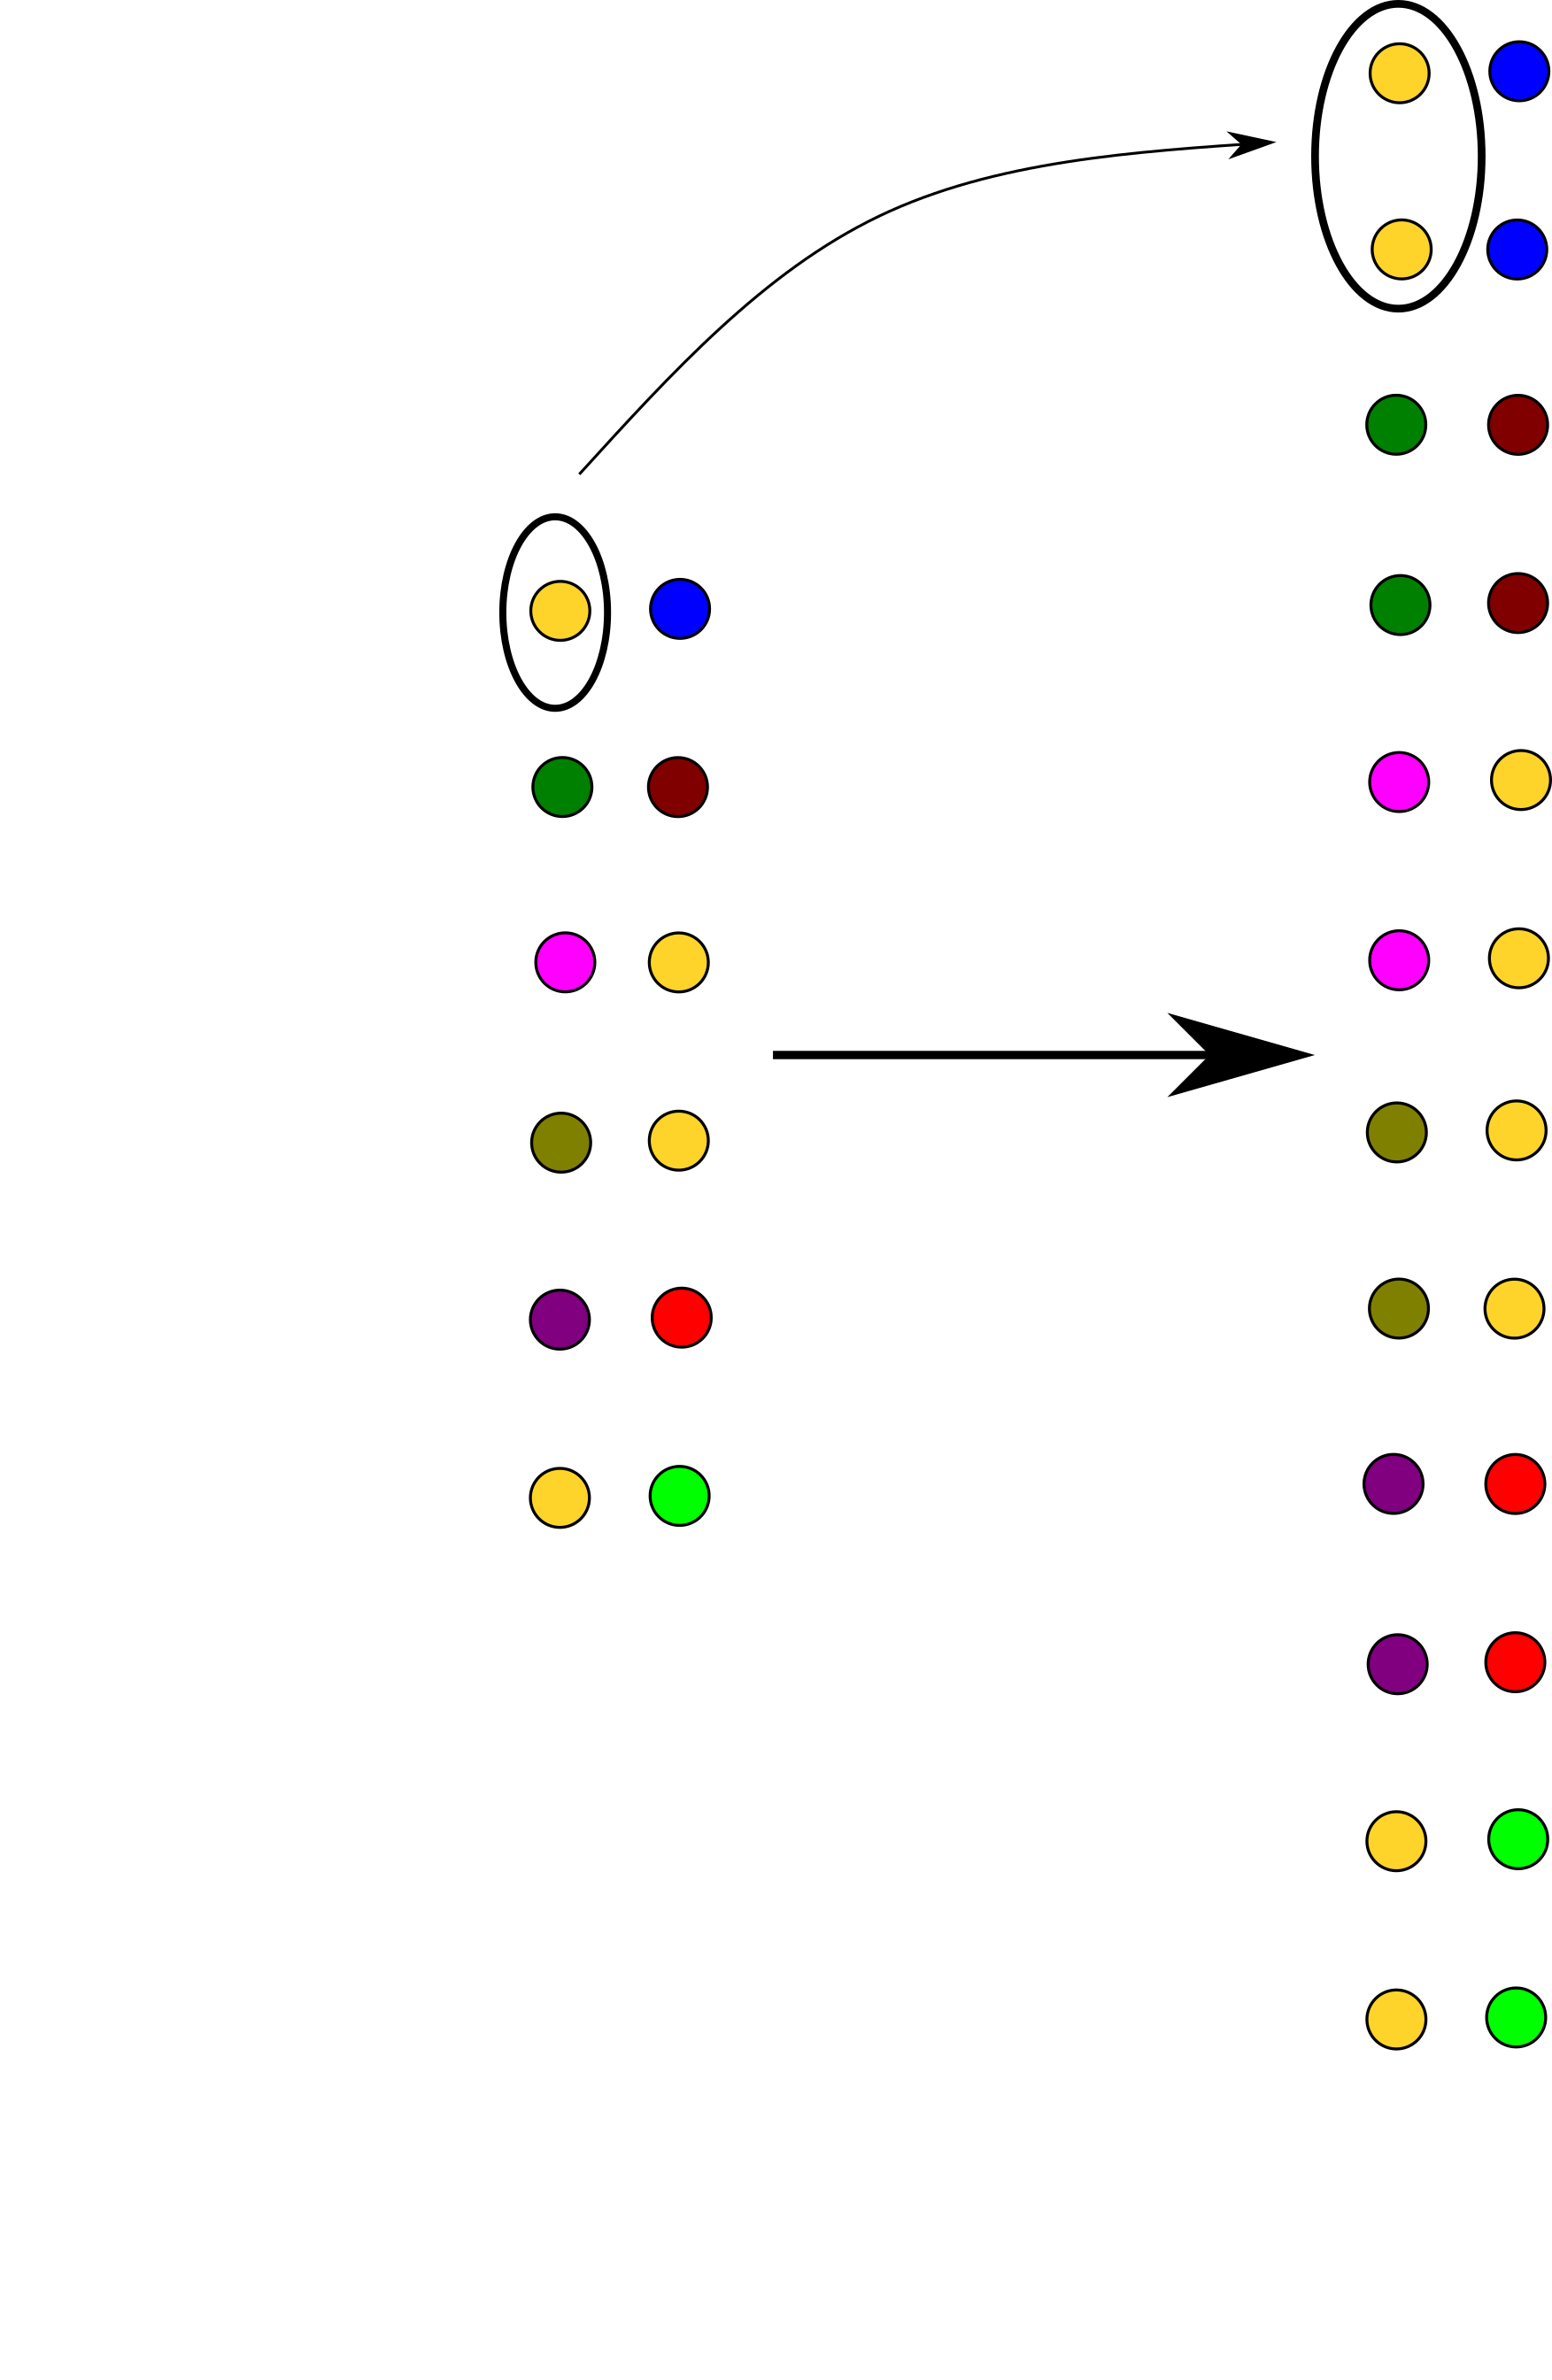
\includegraphics[height=\textheight]{upsampling.png}
    \end{figure}

\end{frame}


%%%%%%%%%%%%%%%%%%%%%%%%%%%%%%%%%%%%
\begin{frame}{Pooling index memorization}

\end{frame}


%%%%%%%%%%%%%%%%%%%%%%%%%%%%%%%%%%%%
\begin{frame}{Transposed convolution}

\end{frame}


%%%%%%%%%%%%%%%%%%%%%%%%%%%%%%%%%%%%%%%%%%%%%%%%%%%%%
\section[Properties]{Properties of fully-convolutional neural networks}

%%%%%%%%%%%%%%%%%%%%%%%%%%%%%%%%%%%%%%%%%%%%%%%%%%%%%
\subsection{Receptive field}
%%%%%%%%%%%%%%%%%%%%%%%%%%%%%%%%%%%%%%%%%%%%%%%%%%
\frame{
  \frametitle{Receptive field}

  \begin{block}{Definition: links between neurons}
    In a NN, we say that neuron $a$ is linked to neuron $b$ if there is an oriented path in the corresponding graph going from $a$ to $b$.
  \end{block}


  \begin{block}{Definition}
    The \alert{receptive field} of a neuron in a NN is the set of \emph{input neurons} that are linked to that neuron.

    The size of the receptive field is an essential property when designing a fully-convolutional NN architecture.
  \end{block}

}

%%%%%%%%%%%%%%%%%%%%%%%%%%%%%%%%%%%%
\begin{frame}<beamer>{Illustration}

  \begin{figure}
    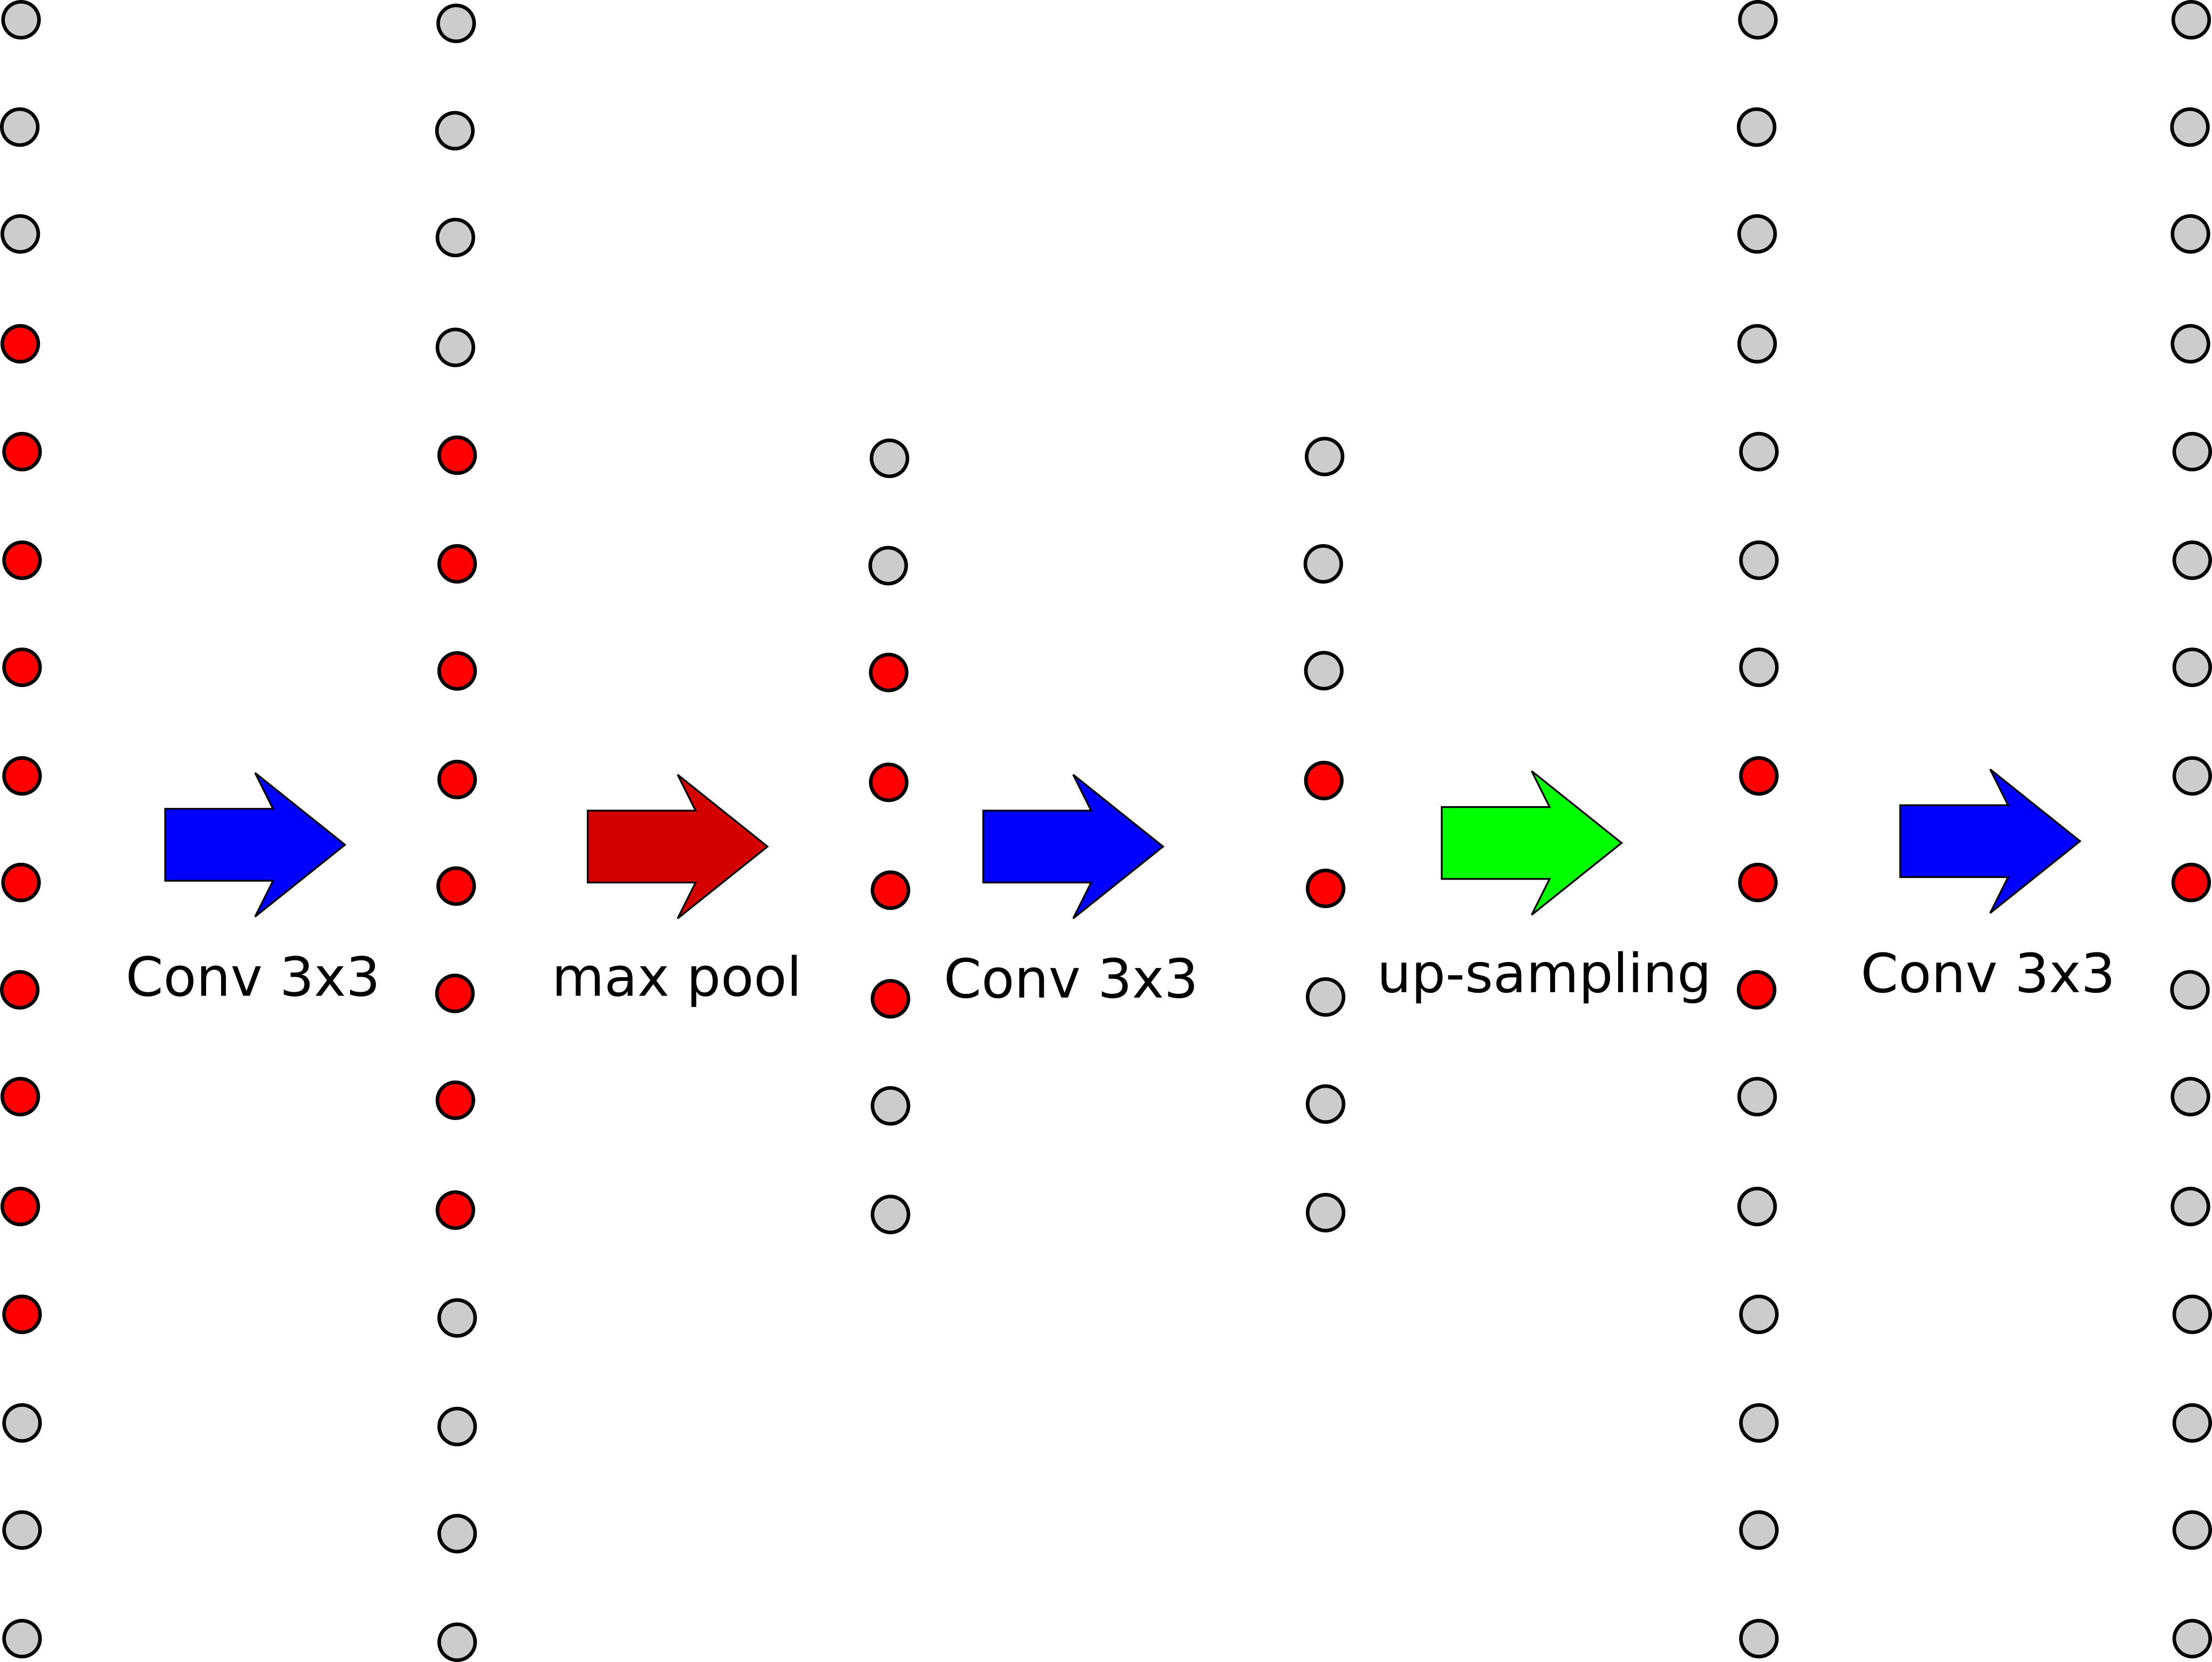
\includegraphics[width=0.8\textwidth]{receptive_field.png}
  \end{figure}

\end{frame}

%%%%%%%%%%%%%%%%%%%%%%%%%%%%%%%%%%%%
\begin{frame}{Illustration}

  \begin{figure}
  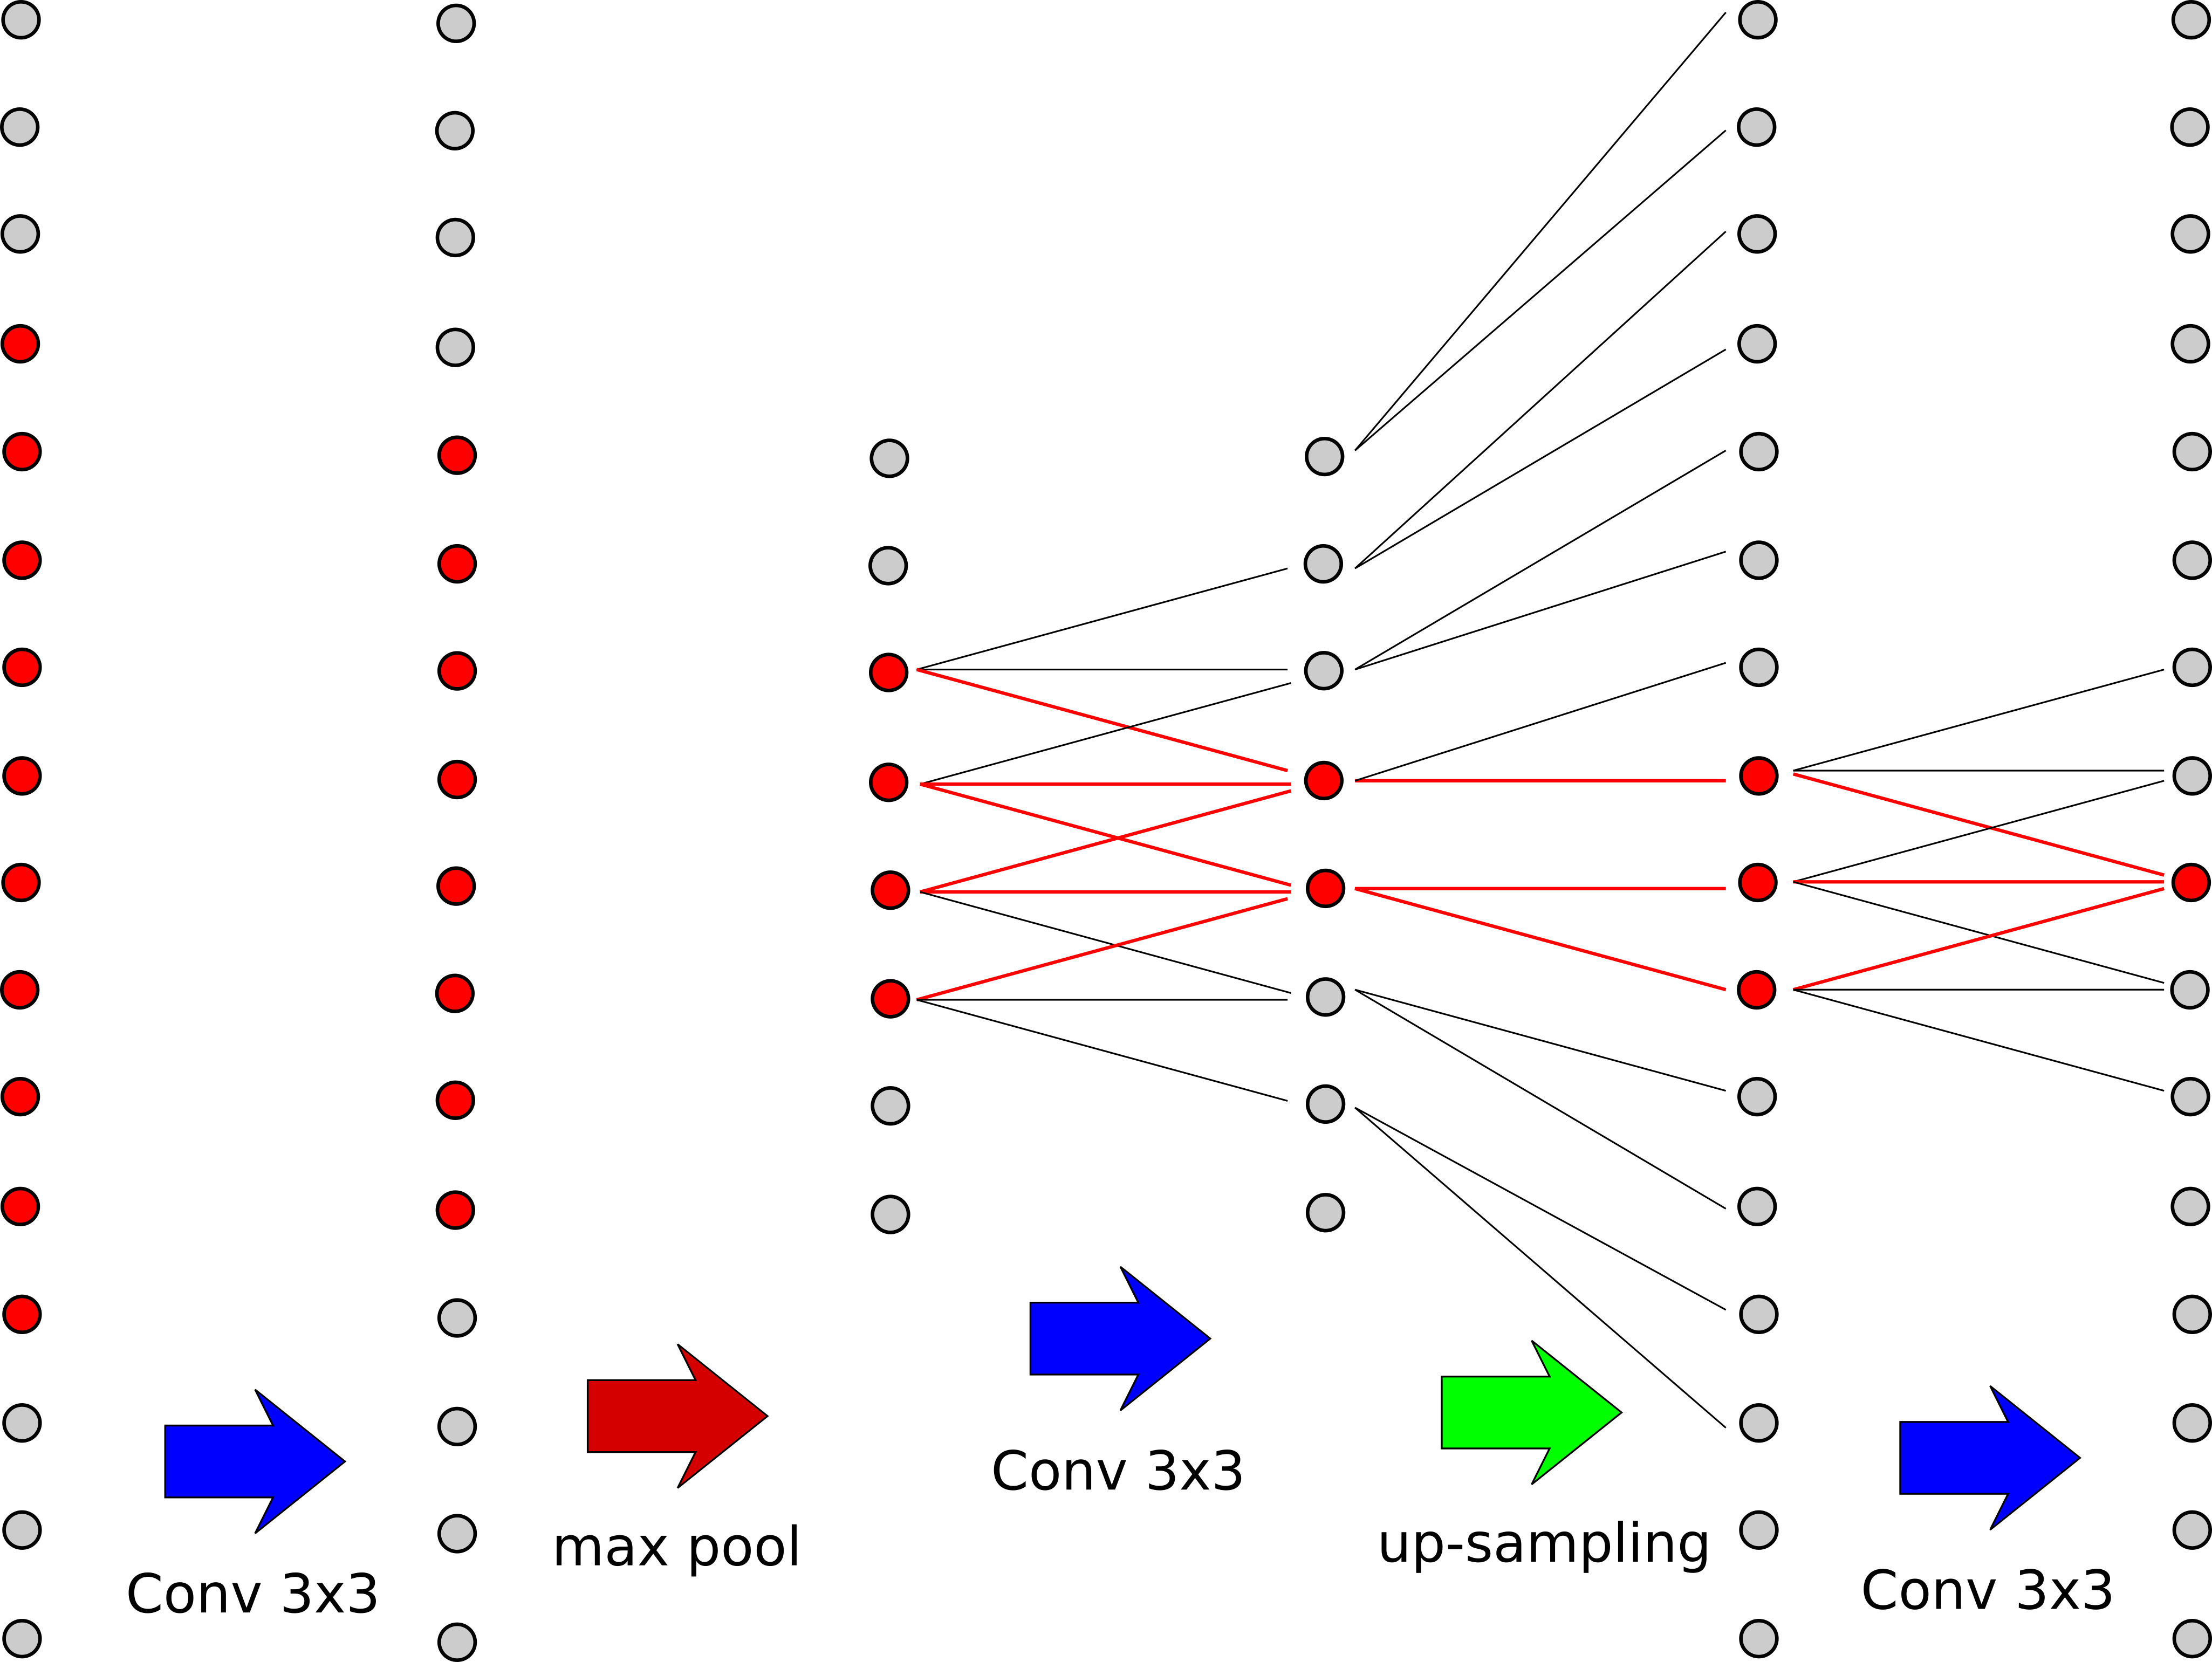
\includegraphics[width=0.8\textwidth]{receptive_field2.png}
  \end{figure}

\end{frame}

%%%%%%%%%%%%%%%%%%%%%%%%%%%%%%%%%%%%
\begin{frame}{Receptive field evolution through an upsampling layer}

  \begin{figure}
  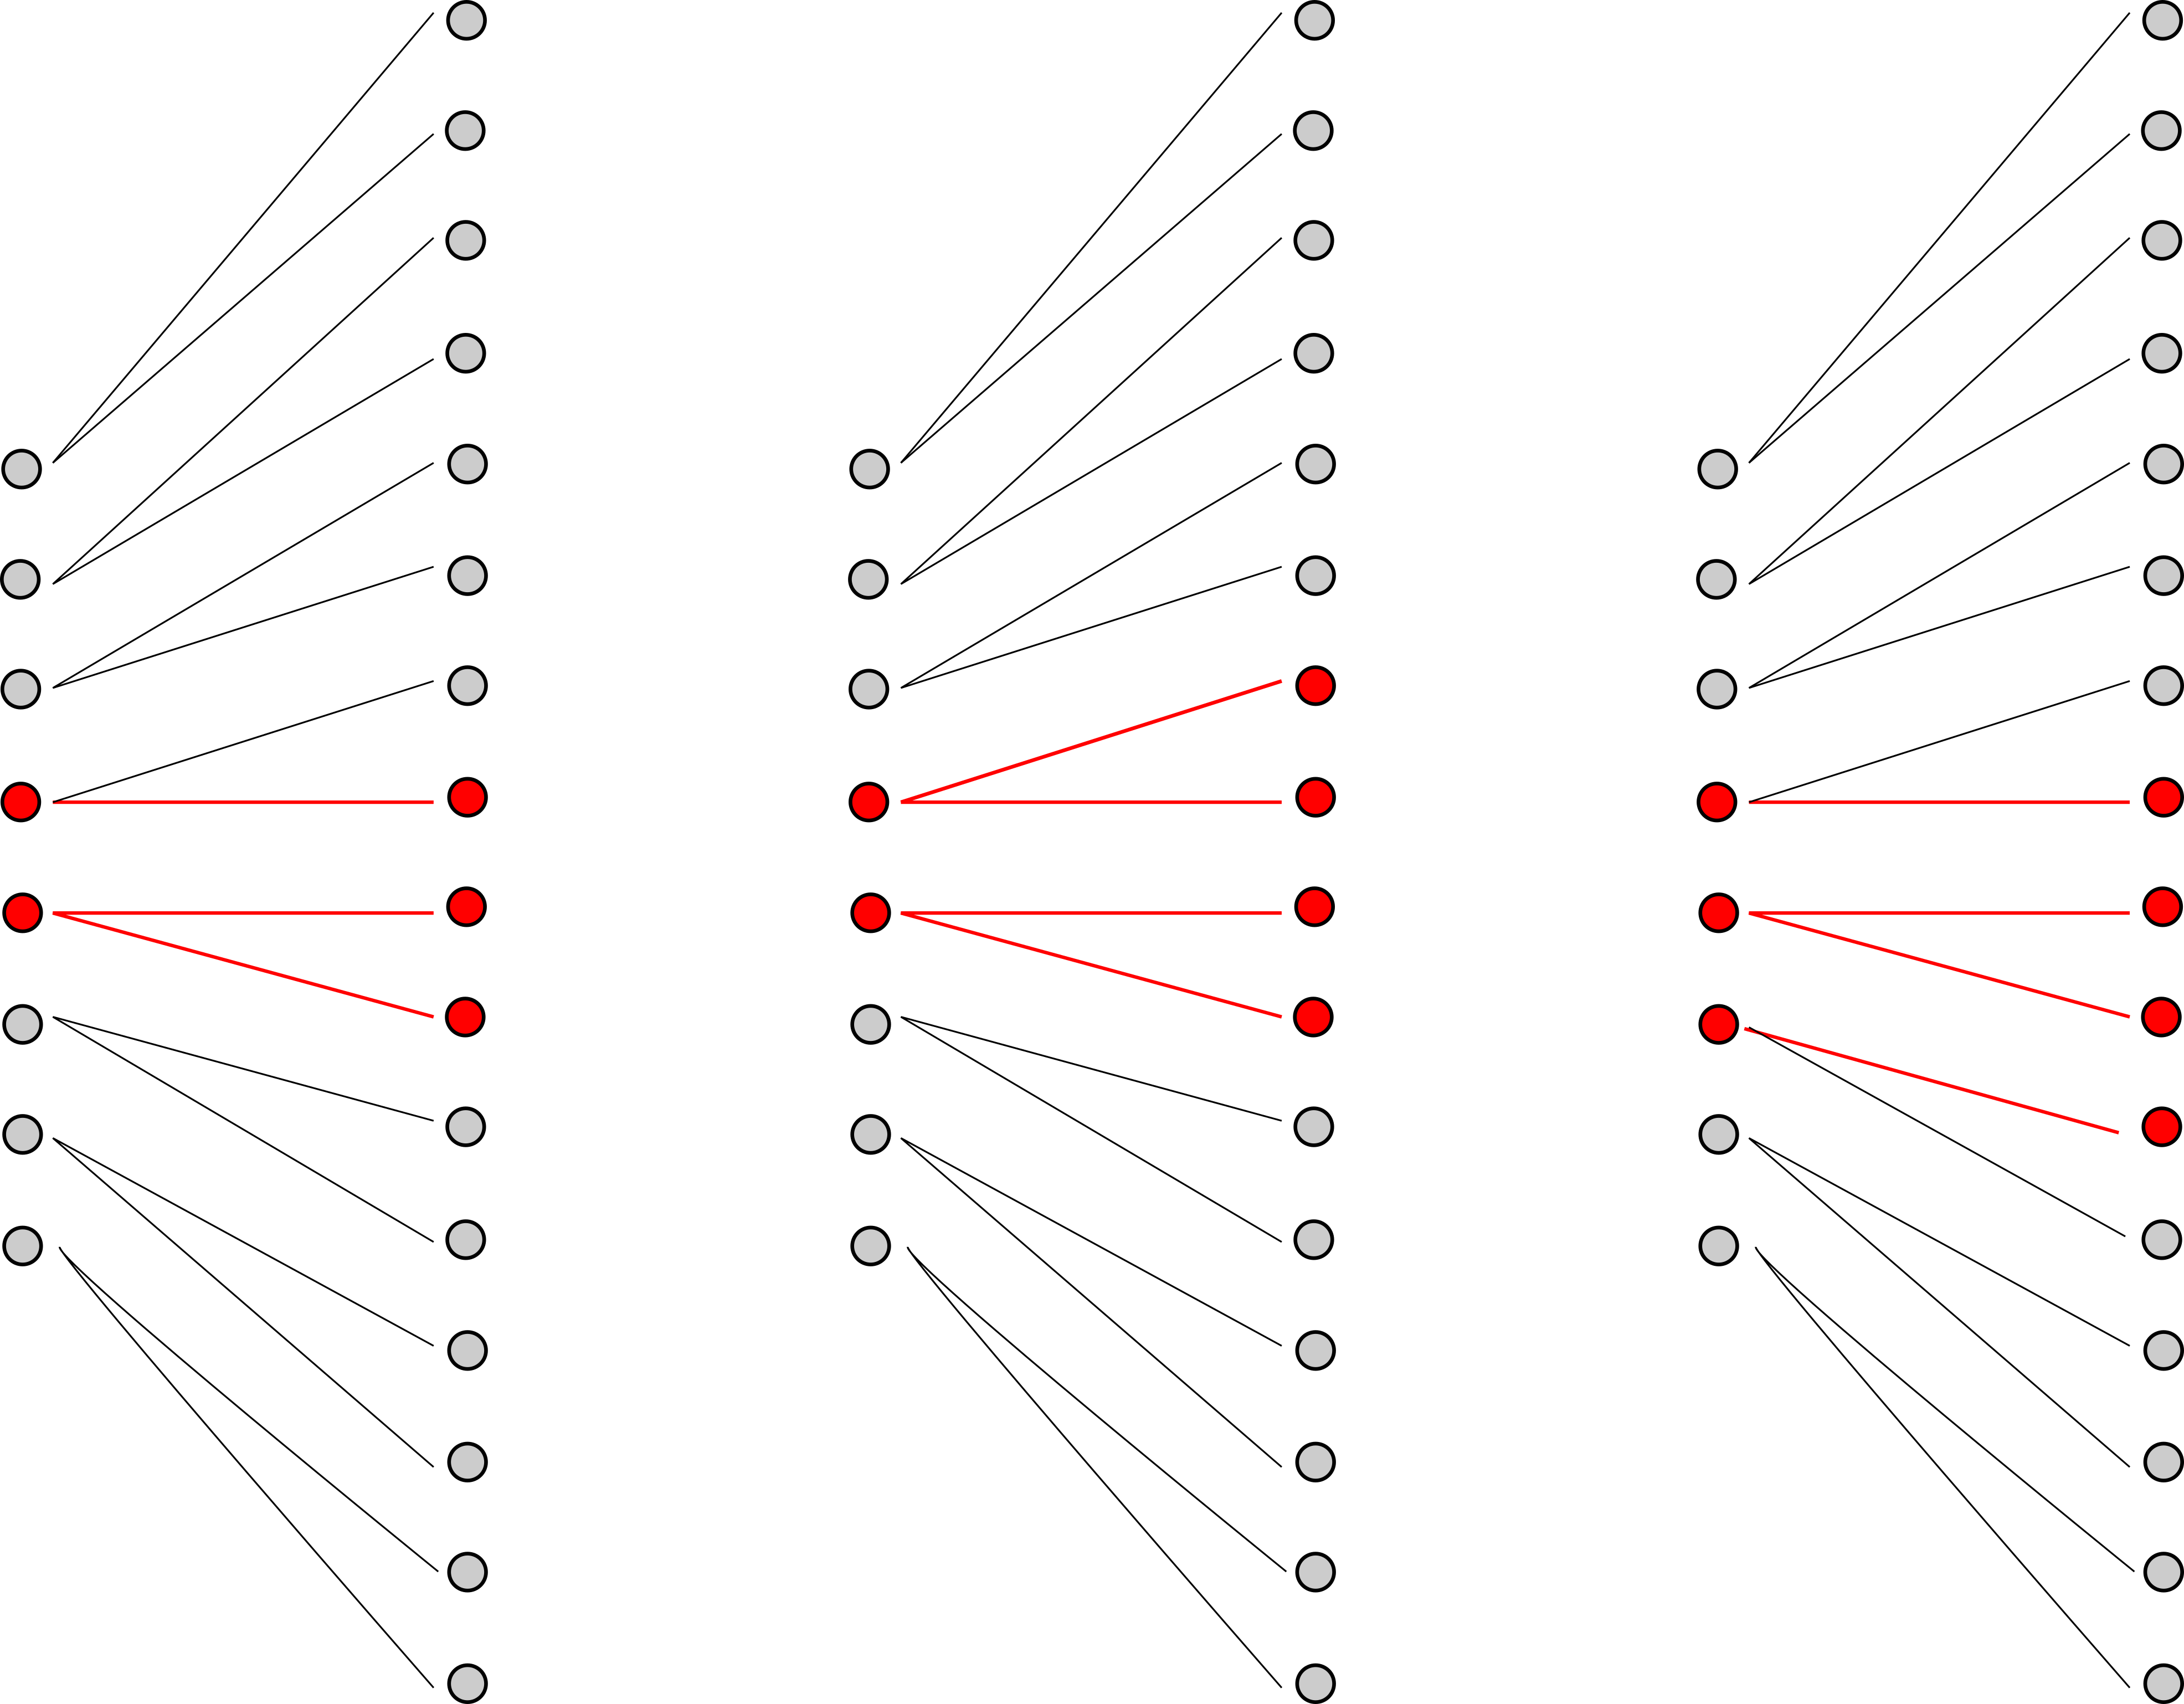
\includegraphics[width=0.8\textwidth]{receptive_field_upsampling.png}
  \end{figure}

\end{frame}

%%%%%%%%%%%%%%%%%%%%%%%%%%%%%%%%%%%%%%%%%%%%%%%%%%
\frame<beamer>{
  \frametitle{Example}

  \begin{block}{What is the size of the receptive field of the neurons in the last layer?}
    \begin{figure}
      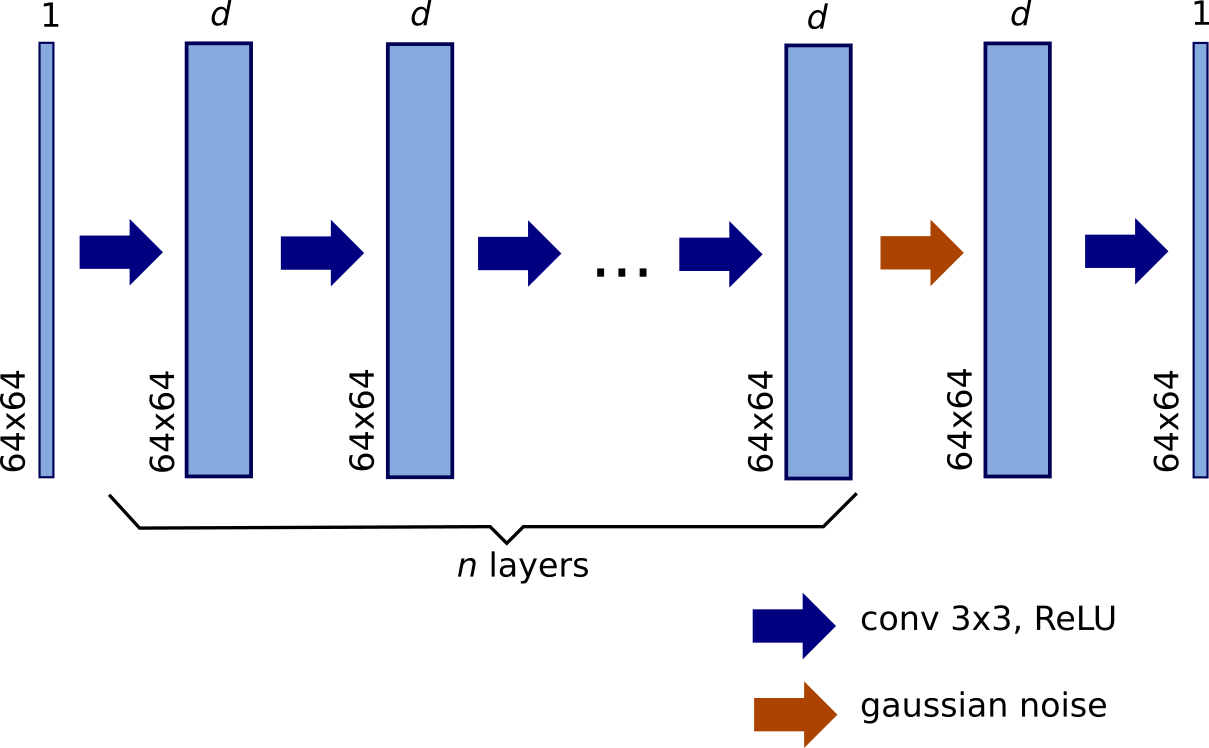
\includegraphics[width=\textwidth]{plain_convnet.png}
    \end{figure}
  \end{block}

  \vspace{1em}

  \pause

  \centering
  Answer: $1 + 2 \times (n+1)$

}
%%%%%%%%%%%%%%%%%%%%%%%%%%%%%%%%%%%%%%%%%%%%%%%%%%
\frame<handout>{
  \frametitle{Example}

  \begin{block}{What is the size of the receptive field of the neurons in the last layer?}
    \begin{figure}
      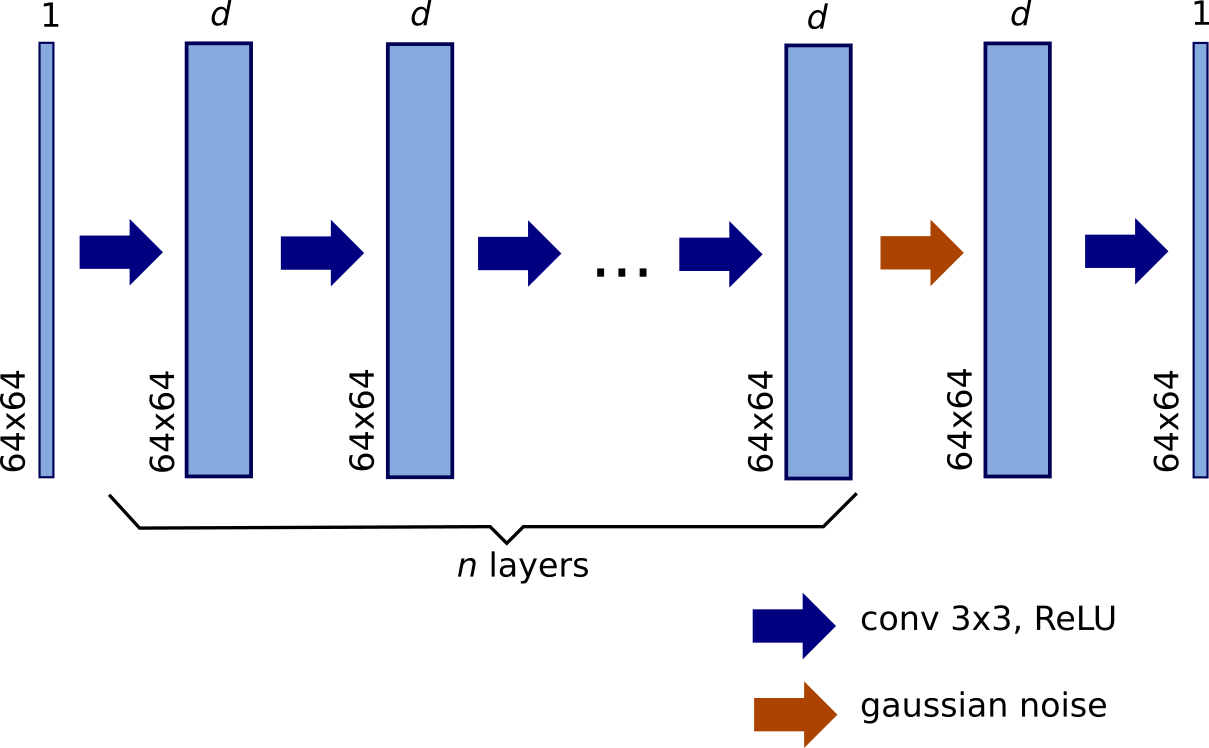
\includegraphics[width=\textwidth]{plain_convnet.png}
    \end{figure}
  \end{block}
}

%%%%%%%%%%%%%%%%%%%%%%%%%%%%%%%%%%%%%%%%%%%%%%%%%%%%%
\subsection{Translation equivariance}

%%%%%%%%%%%%%%%%%%%%%%%%%%%%%%%%%%%%
\begin{frame}{Equivariance}

\begin{block}{Definition}
  A function $f: E \longrightarrow F$ if equivariant with respect to the functions $t_E: E \longrightarrow E$ and $t_F: F \longrightarrow F$ iff $\forall x \in E$:
  \[
  f(t_E(x)) = t_F(F(x))
  \]
\end{block}

\end{frame}

%%%%%%%%%%%%%%%%%%%%%%%%%%%%%%%%%%%%
\begin{frame}{Translation equivariance}

\begin{itemize}
  \item When $E=F$ and $t_E$ and $t_F$ are the same, any, translation, then we have \emph{translation equivariance}.
\item Translation equivariance is an often sought property for image processing operators.
\item Note that we often abusively say \emph{invariant} to translation instead of \emph{equivariant} to translation.
\item Given that in all practical cases images are defined on a bounded set, this property is only true ``far enough'' from the borders
\end{itemize}

\end{frame}

%%%%%%%%%%%%%%%%%%%%%%%%%%%%%%%%%%%%
\begin{frame}{Translation equivariance applied to neural networks}

\begin{block}{Definition}
  Let us consider an operator $f$ between two layers $L_1$ and $L_2$ of a NN. Suppose that the receptive field of this operator for a given neuron $p$ of $L_2$ is $R(p)$, a subset of neurons of $L_1$. Then $f$ is said to be translation equivariant if, for any two neurons $p$ and $q$ of $L_2$, such that $L_1(R(p)) = L_1(R(q))$ (i.e. their receptive fields are identical) then $f(p) = f(q)$.
\end{block}

\begin{alertblock}{}
  Simply put, the operator is translation equivariant if identical receptive fields produce identical values.
\end{alertblock}

\end{frame}

%%%%%%%%%%%%%%%%%%%%%%%%%%%%%%%%%%%%
\begin{frame}{Translation equivariant operators}

\begin{table}[]
\begin{tabular}{|l|l|}
\hline
\textbf{Operator}        & \textbf{Translation equivariant} \\ \hline
Convolution (stride$=1$)             & \onslide<2->{yes}                            \\ \hline
Downsampling (stride $>1$)            & \onslide<3->{no}                             \\ \hline
Transposed convolution (stride$>1$)   & \onslide<4->{yes}                            \\ \hline
Upsampling (stride$>1$) & \onslide<5->{no}                             \\ \hline
Concatenation            & \onslide<6->{yes}                            \\ \hline
Addition                 & \onslide<7->{yes}                            \\ \hline
\end{tabular}
\end{table}

\end{frame}

%%%%%%%%%%%%%%%%%%%%%%%%%%%%%%%%%%%%
\begin{frame}{Translation equivariance}

  \begin{block}{}
    Identical receptive fields produce identical outputs.
  \end{block}

  \pause

  \begin{itemize}[<+->]
  \item If padding is used in the network, border effects can be important.
  \item Translation equivariance is not always welcome!
  \item Position information can also be used in the network:
    \begin{itemize}
    \item Through masks or segmentations
    \item Through pixel coordinates
    \end{itemize}
  \end{itemize}

\end{frame}

%%%%%%%%%%%%%%%%%%%%%%%%%%%%%%%%%%%%
\begin{frame}{Illustration}

\begin{figure}[ht]
  \centering
  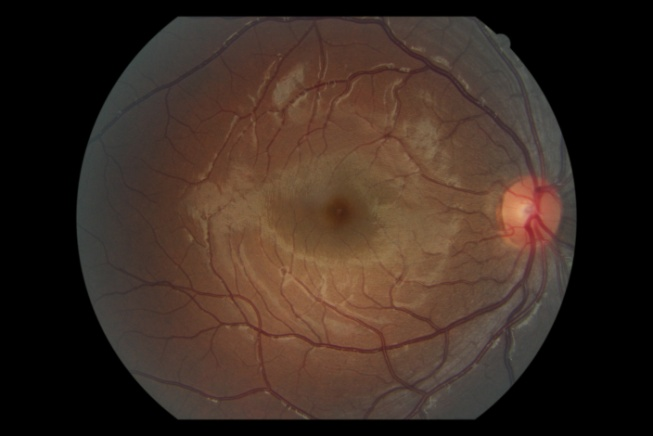
\includegraphics[height=0.8\textheight]{fundus1}
  \caption{Eye fundus / retina image}
  \source{OPHDIAT database}
\end{figure}

\end{frame}


\begin{frame}{Illustration}

\begin{figure}[ht]
  \centering
  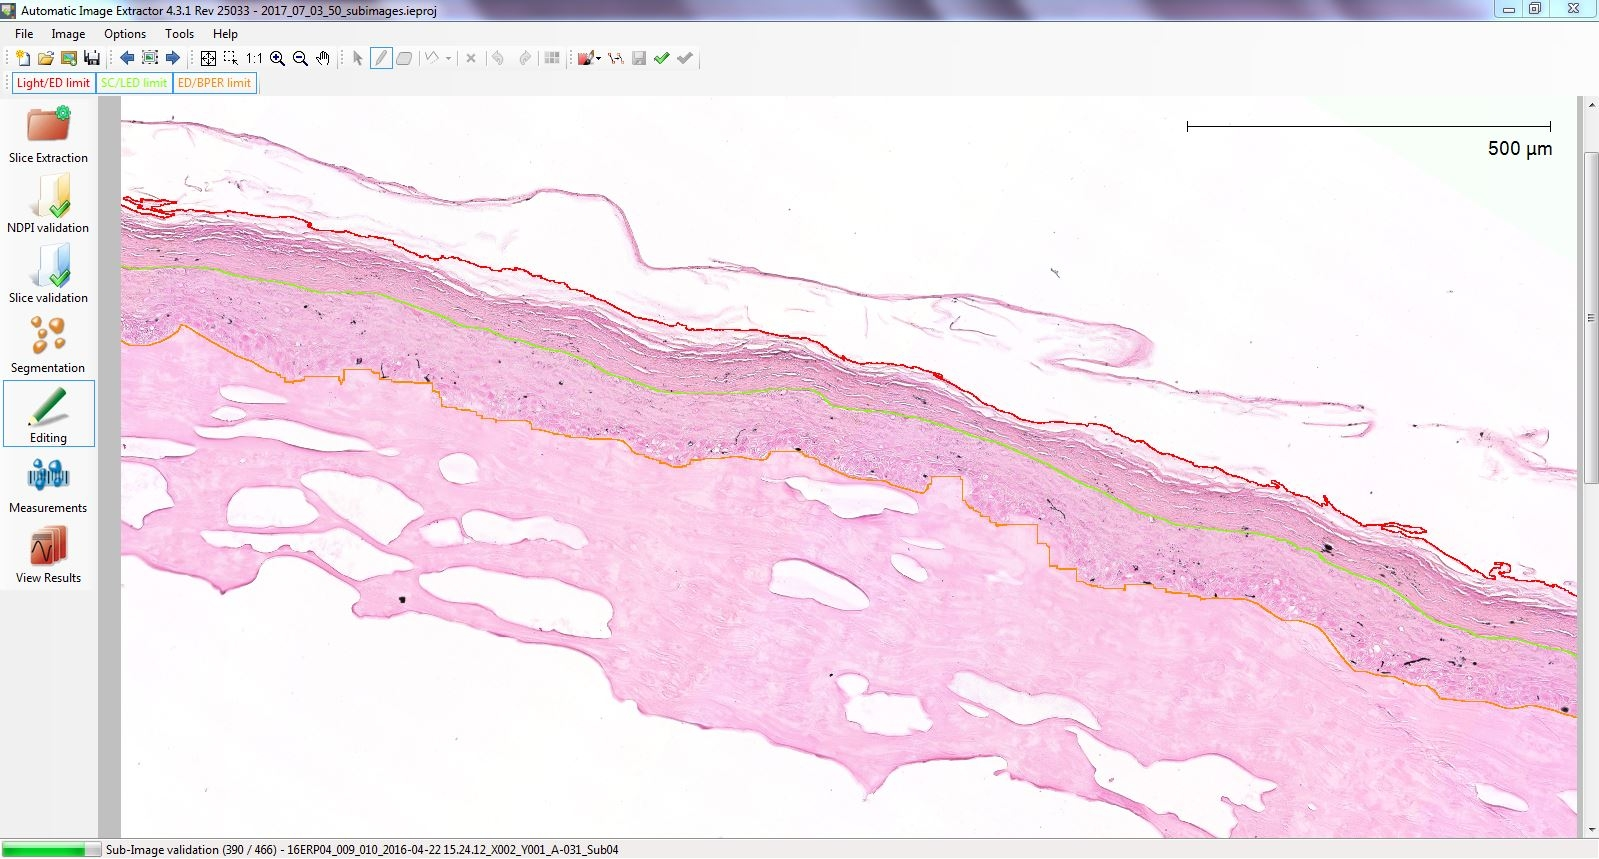
\includegraphics[width=\textwidth]{skin}
  \caption{Histological image of reconstructed skin}
  \source{L'Oréal}
\end{figure}


\end{frame}


%%%%%%%%%%%%%%%%%%%%%%%%%%%%%%%%%%%%%%%%%%%%%%%%%%%%%
\subsection{Other properties}
%%%%%%%%%%%%%%%%%%%%%%%%%%%%%%%%%%%%%%%%%%%%%%%%%%%%%
\frame{
  \frametitle{Image size flexibility}

  \begin{itemize}
  \item A NN containing fully-connected layers can only process images of a given size
  \item A fully convolutional NN can be applied to images of any size, as long as its dimensions are compatible with the subsampling steps of the network
  \item Practical limit: the memory of the system
    \pause
  \item Note that as the input image gets larger, border effects become proportionally less present
  \end{itemize}

}

%%%%%%%%%%%%%%%%%%%%%%%%%%%%%%%%%%%%%%%%%%%%%%%%%%%%%
\frame{
  \frametitle{Robustness with respect to ground-truth errors}

  \begin{block}{}
    This is more an empirical observation than a mathematical property, but fully-convolutional NNs tend to be robust with respect to errors in the contours position on the ground-truth.
  \end{block}


}


%%%%%%%%%%%%%%%%%%%%%%%%%%%%%%%%%%%%%%%%%%%%%%%%%%
\section{Image segmentation}

%%%%%%%%%%%%%%%%%%%%%%%%%%%%%%%%%%%%%%%%%%%%%%%%%%
\frame{
  \frametitle{The specific case of image segmentation}

  \begin{block}{Definition: image segmentation}
    Let $I$ be an image defined on $D$. A segmentation of $I$ is a partition of $D$. In practice the regions of the segmentation should correspond to the objects in $I$, which is application dependant.
  \end{block}


  \begin{itemize}

  \item A partition is often represented as a labelled image

  \item In order to make the segments symmetric, each one is represented by a different channel

  \end{itemize}

  \begin{block}{Image segmentation example}
    \begin{figure}
      \centering
      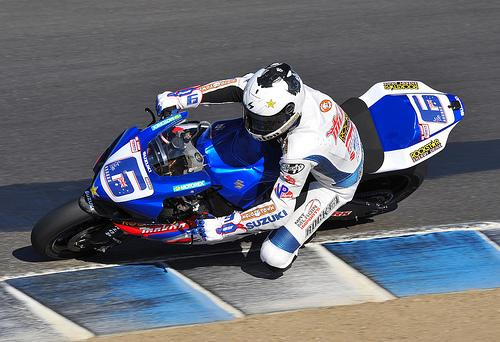
\includegraphics[height=2.5cm]{pascal_moto}
      \hspace{1em}
      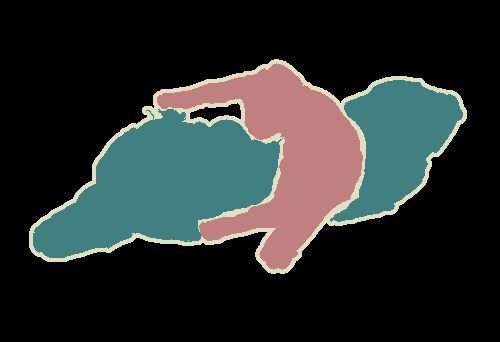
\includegraphics[height=2.5cm]{pascal_moto_seg}\\
      \source{Pascal VOC database}
    \end{figure}
  \end{block}

}

%%%%%%%%%%%%%%%%%%%%%%%%%%%%%%%%%%%%%%%%%%%%%%%%%%
\frame{
  \frametitle{Some vocabulary on segmentation}

  \begin{itemize}

  \item \textbf{Object detection / localization}: bounding box around the object(s).
  \item \textbf{Binary segmentation}: segmentation in 2 classes, background and object.
  \item \textbf{Semantic segmentation}: a label is given to each pixel, according to the object it belongs to.
  \item \textbf{Instance segmentation}: identify each separate object, even if they belong to the same class.

  \end{itemize}

}
%%%%%%%%%%%%%%%%%%%%%%%%%%%%%%%%%%%%%%%%%%%%%%%%%%
% \section{Image segmentation}
%%%%%%%%%%%%%%%%%%%%%%%%%%%%%%%%%%%%%%%%%%%%%%%%%%
\subsection{Binary segmentation}

%%%%%%%%%%%%%%%%%%%%%%%%%%%%%%%%%%%%%%%%%%%%%%%%%%%%%
\frame{
  \frametitle{Neuron membrane segmentation challenge (ISBI 2012)}

  \begin{itemize}
  \item Train: single stack of size $30\times512\times512$.
  \item Test: a second stack of same size.
  \end{itemize}

  \begin{figure}
    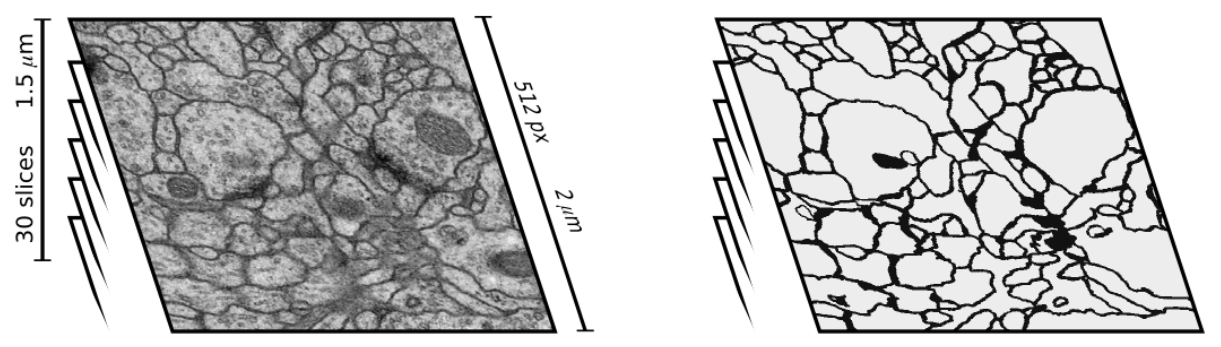
\includegraphics[width=9cm]{em_challenge}
  \end{figure}

}

%%%%%%%%%%%%%%%%%%%%%%%%%%%%%%%%%%%%%%%%%%%%%%%%%%%%%
\frame{
  \frametitle{Neuron membrane segmentation challenge winner~\cite{ciresan_deep_2012}}

  \begin{figure}
    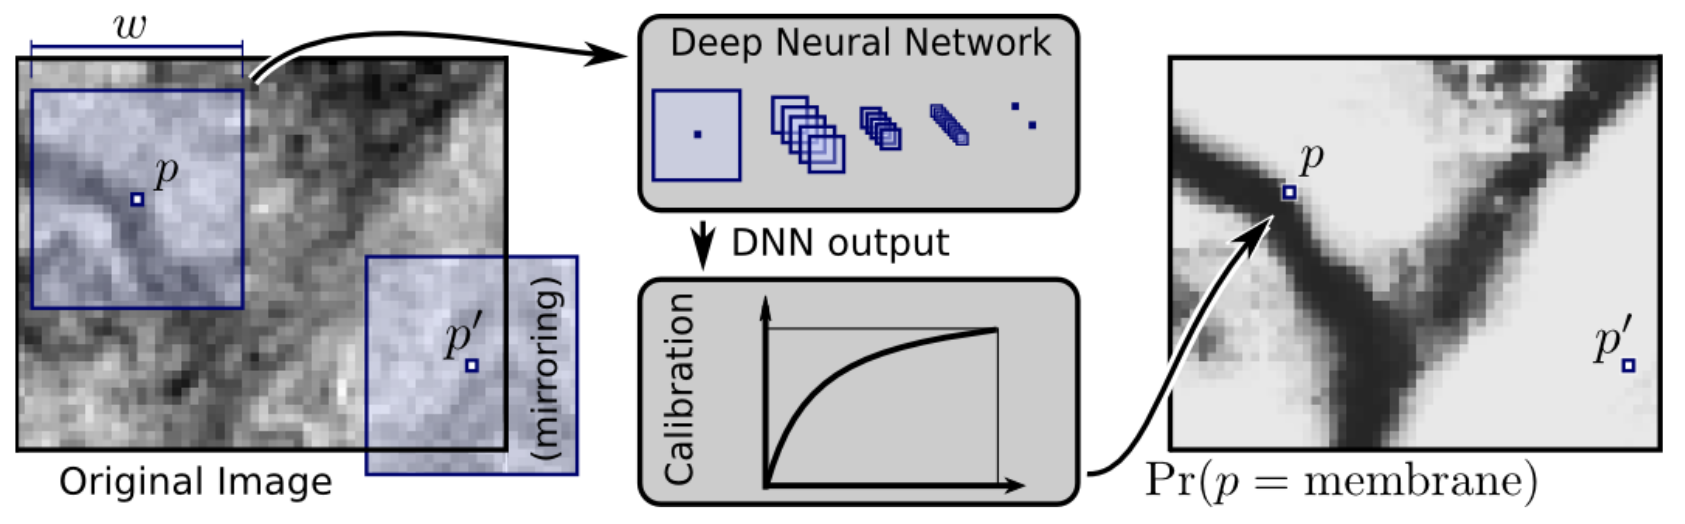
\includegraphics[width=9cm]{dnn_ciresan}
  \end{figure}

}

%%%%%%%%%%%%%%%%%%%%%%%%%%%%%%%%%%%%%%%%%%%%%%%%%%
%%%%%%%%%%%%%%%%%%%%%%%%%%%%%%%%%%%%%%%%%%%%%%%%%%
\subsection{Semantic segmentation}


%%%%%%%%%%%%%%%%%%%%%%%%%%%%%%%%%%%%%%%%%%%%%%%%%%%%%
\frame{
  \frametitle{Pascal visual object classes segmentation challenge 2012 \cite{everingham_pascal_2014}}

  \begin{itemize}
  \item 1464 training and 1449 validation images
  \item automatic online test, with unknown images
  \item 20 image categories (cat, sofa, motorbike, person, etc.)
  \end{itemize}

  \begin{figure}
    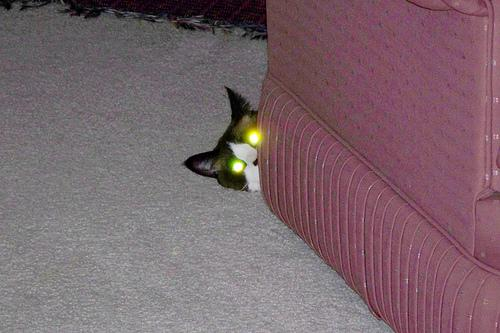
\includegraphics[height=2.5cm]{pascal_cat}
    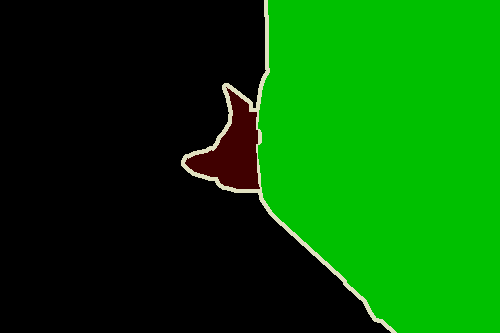
\includegraphics[height=2.5cm]{pascal_cat_seg}\\
    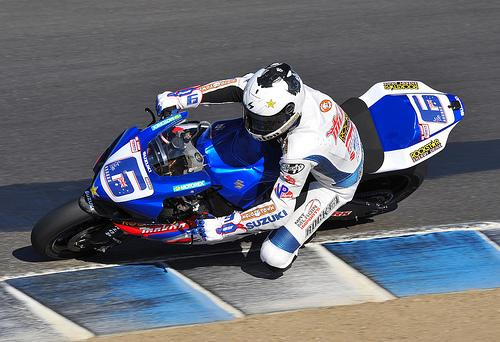
\includegraphics[height=2.5cm]{pascal_moto}
    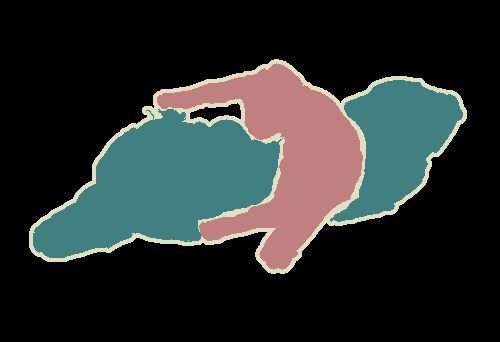
\includegraphics[height=2.5cm]{pascal_moto_seg}
  \end{figure}

}

%%%%%%%%%%%%%%%%%%%%%%%%%%%%%%%%%%%%%%%%%%%%%%%%%%%%%

\frame{
  \frametitle{Convolutional nets for semantic image segmentation}

  Three papers in 2015:

  \begin{itemize}

  \item Fully convolutional networks for semantic segmentation \cite{long_fully_2015}
  \item U-Net: convolutional networks for biomedical image segmentation \cite{ronneberger_u-net:_2015}
  \item SegNet: A Deep Convolutional Encoder-Decoder Architecture for Image Segmentation \cite{badrinarayanan_segnet:_2015}

  \end{itemize}

}

%%%%%%%%%%%%%%%%%%%%%%%%%%%%%%%%%%%%%%%%%%%%%%%%%%
\frame{
  \frametitle{Example: U-Net architecture \cite{ronneberger_u-net:_2015}}

  \begin{figure}
    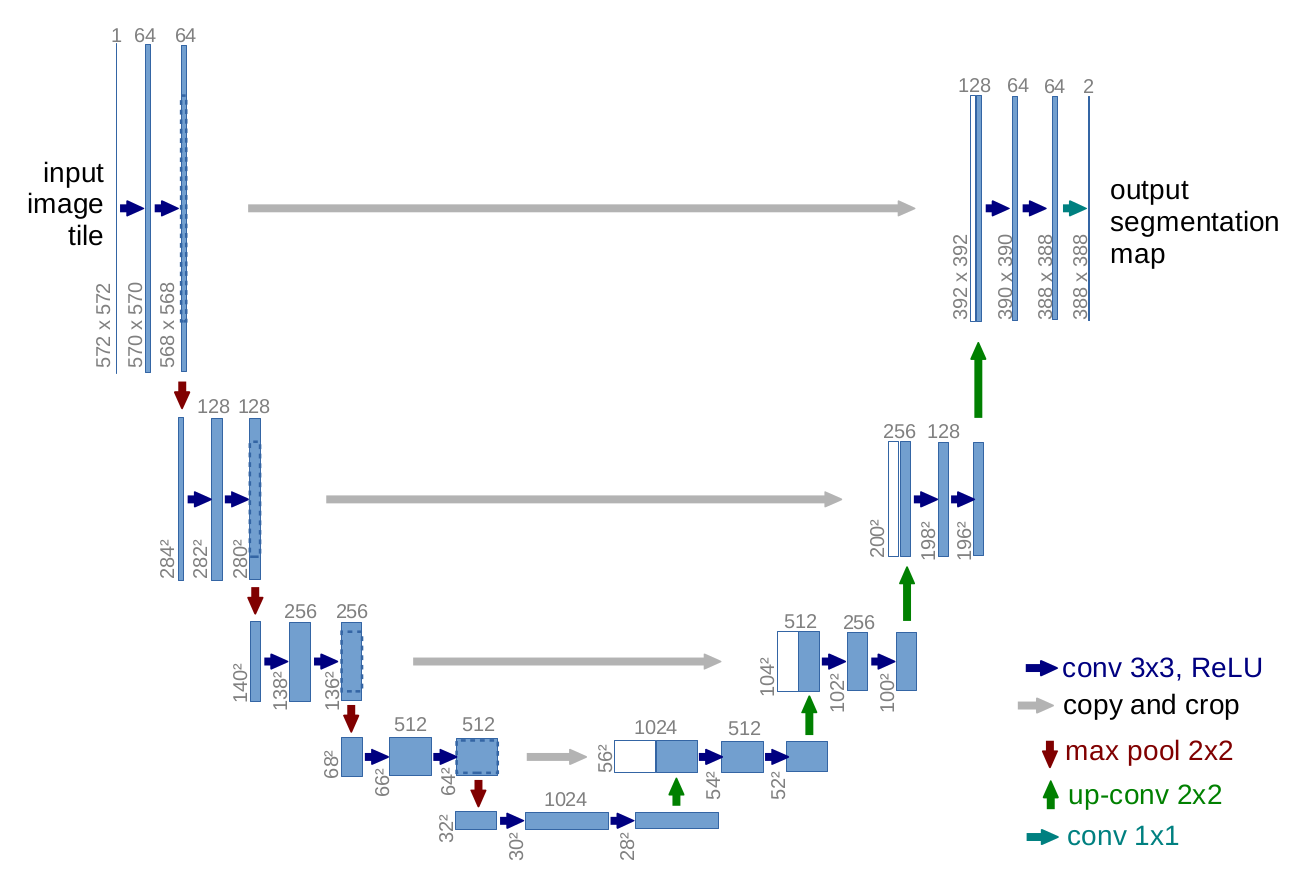
\includegraphics[height=7cm]{unet}
  \end{figure}
}



%%%%%%%%%%%%%%%%%%%%%%%%%%%%%%%%%%%%%%%%%%%%%%%%%%
\frame{
  \frametitle{Example: SegNet architecture \cite{badrinarayanan_segnet:_2015}}

  \begin{figure}
    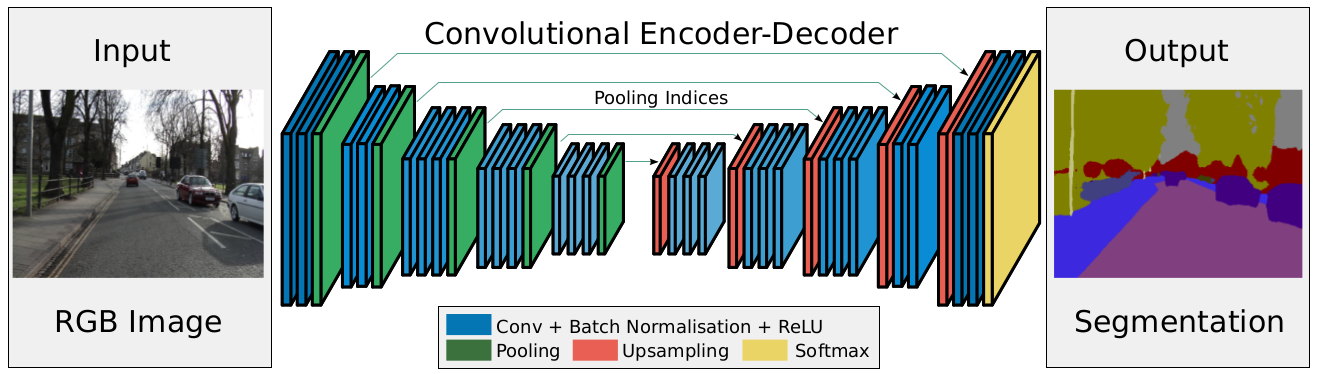
\includegraphics[width=9cm]{segnet_archi}
  \end{figure}
}

%%%%%%%%%%%%%%%%%%%%%%%%%%%%%%%%%%%%%%%%%%%%%%%%%%

\frame{
  \frametitle{Remarks}

  \begin{itemize}
  \item These architectures easily contain a number of parameters of the order of $10^7$ (28 million for U-Net)
  \item Their optimization might be difficult
  \item But you can reduce the number of filters or the number of layers

  \end{itemize}

}

%%%%%%%%%%%%%%%%%%%%%%%%%%%%%%%%%%%%%%%%%%%%%%%%%%%%%
%%%%%%%%%%%%%%%%%%%%%%%%%%%%%%%%%%%%%%%%%%%%%%%%%%%%%
\subsection{Instance segmentation}
%%%%%%%%%%%%%%%%%%%%%%%%%%%%%%%%%%%%%%%%%%%%%%%%%%

\frame{
  \frametitle{COCO: common objects in context \cite{lin_microsoft_2014}}

  \begin{itemize}
  \item $2$ million objects, from $80$ categories, in $300\,000$ images
  \end{itemize}


  \begin{figure}
    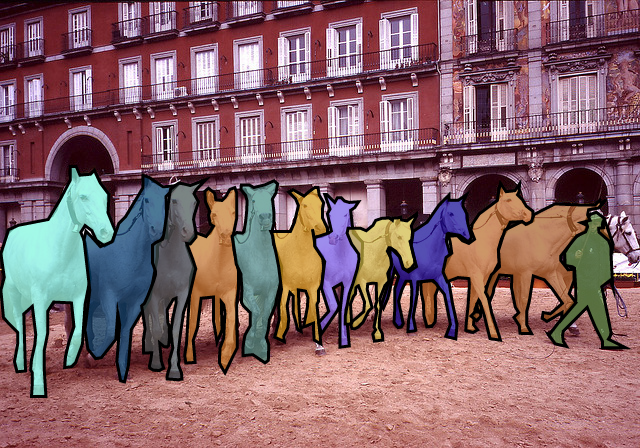
\includegraphics[height=3.4cm]{coco_ex_horses}
    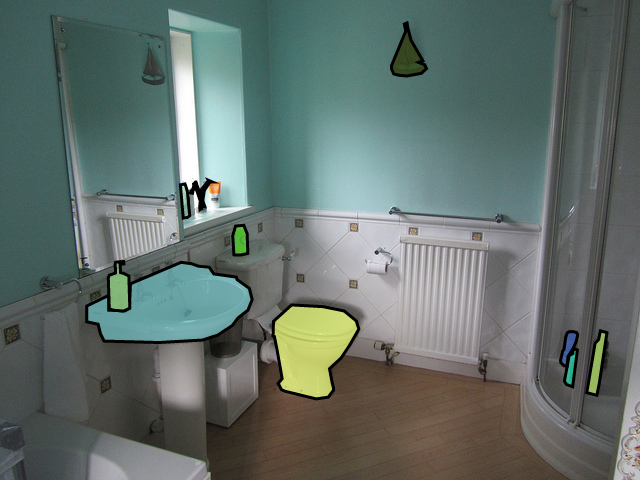
\includegraphics[height=3.4cm]{coco_ex_salle_de_bain}
  \end{figure}

  \begin{block}{}
    Winner 2016: Fully Convolutional Instance-aware Semantic Segmentation (Microsoft) \cite{li_fully_2016}
  \end{block}

}


%%%%%%%%%%%%%%%%%%%%%%%%%%%%%%%%%%%%%%%%%%%%%%%%%%%%%
\frame{
  \frametitle{COCO instance segmentation challenge: examples of 2016 winner results}

  \begin{figure}
    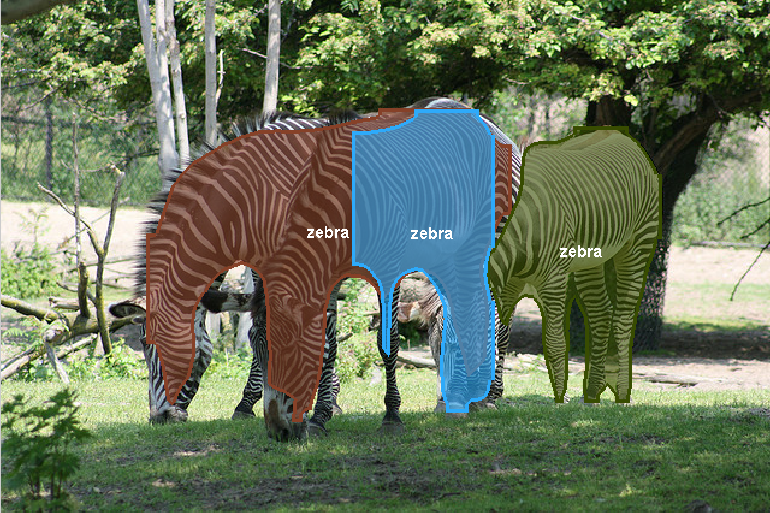
\includegraphics[width=4.5cm]{COCO_test2015_000000003241.png}
    \hspace{1cm}
    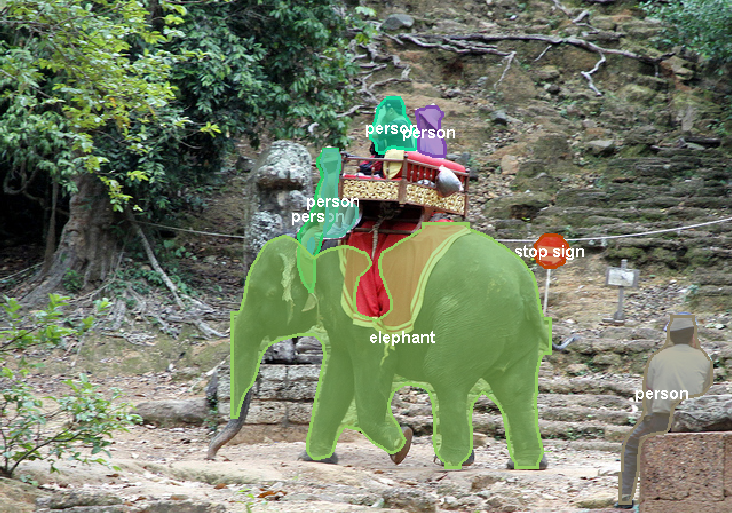
\includegraphics[width=4.5cm]{COCO_test2015_000000004178.png}\\
    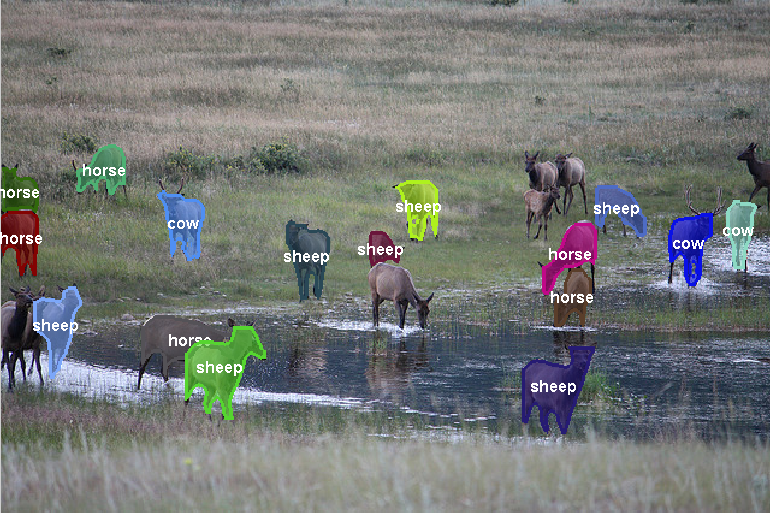
\includegraphics[width=4.5cm]{COCO_test2015_000000006147.png}
    \hspace{1cm}
    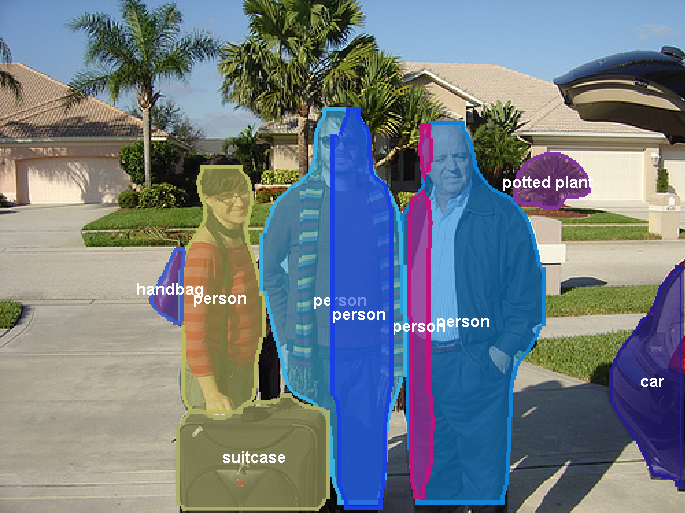
\includegraphics[width=4.5cm]{COCO_test2015_000000016177.png}
  \end{figure}

}

%%%%%%%%%%%%%%%%%%%%%%%%%%%%%%%%%%%%%%%%%%%%%%%%%%%%%
\frame{
  \frametitle{State of the art on the COCO database: Mask R-CNN \cite{he_mask_2017}}

  \begin{figure}
    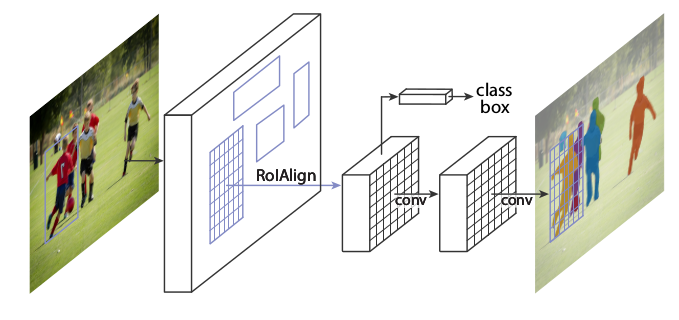
\includegraphics[width=7.5cm]{mask_r_cnn.png}
  \end{figure}
}

%%%%%%%%%%%%%%%%%%%%%%%%%%%%%%%%%%%%%%%%%%%%%%%%%%%%%
\frame{
  \frametitle{Mask R-CNN on the COCO database}

  \begin{figure}
    \includegraphics[width=9cm]{mask_r_cnn_examples.png}
  \end{figure}

}

%%%%%%%%%%%%%%%%%%%%%%%%%%%%%%%%%%%%%%%%%%%%%%%%%%%%%
\frame{
  \frametitle{Partially supervised segmentation - \cite{hu_learning_2017}}

  \begin{itemize}
  \item 80 segmented categories from COCO database (320k images)
  \item 3000 visual concepts using box annotations from the Visual Genome data set (100k images)
  \end{itemize}

  \begin{figure}
    \includegraphics[width=12cm]{segm_every_thing_method.png}
  \end{figure}

}

%%%%%%%%%%%%%%%%%%%%%%%%%%%%%%%%%%%%%%%%%%%%%%%%%%%%%
%% \frame{
%%   \frametitle{Partially supervised segmentation - learning to segment every thing}

%%   \begin{figure}
%%     \includegraphics[width=8cm]{segment_every_thing.png}
%%   \end{figure}

%% \cite{hu_learning_2017}

%%   }

%%%%%%%%%%%%%%%%%%%%%%%%%%%%%%%%%%%%%%%%%%%%%%%%%%
%% \frame{
%%   \frametitle{Current (?) trends for instance segmentation}

%%   \begin{itemize}

%%   \item Region proposal +
%%   \item Fully convolutional (very deep) network +
%%   \item (Post-processing)

%%   \end{itemize}

%%   \begin{figure}
%%     \includegraphics[width=9.5cm]{r_cnn.png}
%%     \caption{Regions with CNN features (R-CNN) (from \cite{girshick_rich_2014})}
%%   \end{figure}

%%   \begin{block}<2->{Meanwhile, on the object detection field...}
%%     \begin{itemize}
%%     \item YOLO: you look only once \cite{redmon_yolo9000:_2016}
%%     \item SSD: single shot detector \cite{liu_ssd:_2016}
%%     \end{itemize}
%%   \end{block}

%% }

%%%%%%%%%%%%%%%%%%%%%%%%%%%%%%%%%%%%%%%%%%%%%%%%%%

%% \frame{
%% \frametitle{A typical convolutional architecture for image classification}

%% \begin{figure}
%%   \includegraphics[width=9.5cm]{conv_net_classif}
%%   \caption{Architecture used for the classification of the NORB dataset (from \cite{scherer_evaluation_2010})}
%% \end{figure}

%% Note that layer P4 can be seen as made of features, which are then classified by the two fully connected layers.


%% }


%%%%%%%%%%%%%%%%%%%%%%%%%%%%%%%%%%%%%%%%%%%%%%%%%%
\section{U-Net}

%%%%%%%%%%%%%%%%%%%%%%%%%%%%%%%%%%%%%%%%%%%%%%%%%%
\frame{
  \frametitle{U-Net architecture \cite{ronneberger_u-net:_2015}}

  \begin{figure}
    \includegraphics[width=\textwidth]{unet_lo}
  \end{figure}

  \begin{itemize}
  \item Size and number of channels of input images?
  \item Segmentation into how many regions?
  \end{itemize}
}

%%%%%%%%%%%%%%%%%%%%%%%%%%%%%%%%%%%%
\begin{frame}{U-Net main ideas}

      \begin{figure}
        \includegraphics[width=0.86\textwidth]{unet_lo}
      \end{figure}


      \begin{itemize}
      \item Encoding branch inspired by classification nets
      \item Decoding branch is symmetrical
      \item Skip connections
      \end{itemize}


\end{frame}


%%%%%%%%%%%%%%%%%%%%%%%%%%%%%%%%%%%%%%%%%%%%%%%%%%
\frame{
  \frametitle{U-Net details}

  \begin{columns}
    \begin{column}{.4\textwidth}
      \begin{figure}
        \includegraphics[width=\textwidth]{unet_lo}
      \end{figure}

    \end{column}

    \begin{column}{.6\textwidth}

      \begin{itemize}
      \item Activation of the last layer: soft-max
      \item Other activations: ReLU
      \item Loss used in the original publication: cross entropy with a weight map $w$ to favor some pixels:
        \[
        L(\param) = \sum\limits_{M \in D} w(M)\log(\hat{y}_{l(M)}(M))
        \]
      \end{itemize}

    \end{column}
  \end{columns}

}

%%%%%%%%%%%%%%%%%%%%%%%%%%%%%%%%%%%%
\begin{frame}{Illustration}

\end{frame}


%%%%%%%%%%%%%%%%%%%%%%%%%%%%%%%%%%%%
\begin{frame}{U-Net improvements}

  \begin{itemize}
  \item Convolutions with stride 2 instead of max-pooling in the encoder
  \item Transposed convolutions instead  of simple up-sampling in the decoder
  \item Using an already optimized classification network as backbone for the encoder
  \end{itemize}

\end{frame}


%%%%%%%%%%%%%%%%%%%%%%%%%%%%%%%%%%%%%%%%%%%%%%%%%%
%% \frame{
%% \frametitle{What is the size of the receptive field of U-Net}


%% \begin{figure}
%% \includegraphics[height=5cm]{unet_lo}
%% \end{figure}

%% \pause

%%   \centering
%%   Answer: $185 \times 185$
%% }



%%%%%%%%%%%%%%%%%%%%%%%%%%%%%%%%%%%%%%%%%%%%%%%%%%
\section[Using CNNs]{Using fully-convolutional networks}



%%%%%%%%%%%%%%%%%%%%%%%%%%%%%%%%%%%%
\begin{frame}{Dealing with image sizes during training}

  \begin{itemize}[<+->]
  \item   In segmentation applications, original images are often of different sizes and possibly very large.
  \item   In theory, given the translation equivariance of fully-convolutional NN, we could use them directly as input. In practice, we are limited by memory size.
  \item   Solution: extract fixed-sized crops from your training set:
    \begin{itemize}
    \item make them as large as possible, to reduce border effects
    \item take a small batch size (1, 2, 4?)
    \end{itemize}

  \end{itemize}

\end{frame}


%%%%%%%%%%%%%%%%%%%%%%%%%%%%%%%%%%%%%%%%%%%%%%%%%%%%%
%% \frame{
%%   \frametitle{Post-processing for segmentation}

%%   \begin {itemize}
%%   \item Superpixels (e.g. \cite{farabet_learning_2013})
%%   \item Conditional random fields
%%   \item Mathematical morphology
%%   \end{itemize}

%% }


%%%%%%%%%%%%%%%%%%%%%%%%%%%%%%%%%%%%%%%%%%%%%%%%%%
\frame{
  \frametitle{Loss functions for image segmentation}


  \begin{itemize}
  \item $\hat{\y} = (\hat{\y}_i)$: network output
  \item $\y = (\y_i)$: binary expected output
  \item We suppose that all $\hat{\y}_i$ are in $[0,1]$
  \item We want the $\hat{\y}$ to be \emph{as close as possible} to $\y$
  \end{itemize}

}


%%%%%%%%%%%%%%%%%%%%%%%%%%%%%%%%%%%%%%%%%%%%%%%%%%
\frame{
  \frametitle{Loss functions for image segmentation}


  \begin{block}{A loss function inherited from image classification}

    \begin{itemize}
    \item Cross-entropy: $ -\sum\limits_i y_i\log(\hat{y}_i)$
    \end{itemize}

  \end{block}

}

%%%%%%%%%%%%%%%%%%%%%%%%%%%%%%%%%%%%%%%%%%%%%%%%%%
\frame{
  \frametitle{Measures used in image processing}

  Let $A$ and $B$ be two sets, not simultaneously empty.

  \begin{columns}
    \begin{column}{.7\textwidth}
      \begin{block}{Dice coefficient}
        \[
        D(A,B) = \frac{2|A \cap B|}{|A|+|B|}
        \]
      \end{block}

      \begin{block}{Jaccard index}
        \[
        J(A,B) = \frac{|A \cap B|}{|A \cup B|}
        \]
      \end{block}


    \end{column}

    \begin{column}{.3\textwidth}
      \includegraphics[width=\textwidth]{Intersection_of_sets_A_and_B}
      \source{Public domain (Wikipedia.org)}
    \end{column}
  \end{columns}


  \begin{block}{Properties}
    \begin{itemize}
    \item $\forall A, B: 0 \leq J(A, B) \leq D(A,B) \leq 1$
    \item If $A=B$, then $D(A,B) = J(A,B) = 1$
    \item If $ A \cap B = \emptyset$, then $D(A,B) = J(A,B) = 0$
    \end{itemize}
  \end{block}

}


%%%%%%%%%%%%%%%%%%%%%%%%%%%%%%%%%%%%%%%%%%%%%%%%%%
\frame{
  \frametitle{Generalization to $[0,1]$}

  $\y$ and $\hat{\y}$ are in $[0,1]^n$, not simultaneously equal to $0$.

  \begin{block}{Dice similarity}
    \[
    D(\y, \hat{\y}) = \frac{2\sum_i y_i\hat{y}_i}{\sum_i y_i + \sum_i \hat{y}_i}
    \]
  \end{block}

  \begin{block}{Jaccard similarity}
    \[
    J(\y, \hat{\y}) = \frac{\sum_i y_i\hat{y}_i}{\sum_i y_i + \sum_i \hat{y}_i - \sum_i y_i\hat{y}_i}
    \]
  \end{block}

}


%%%%%%%%%%%%%%%%%%%%%%%%%%%%%%%%%%%%%%%%%%%%%%%%%%
\frame{
  \frametitle{Corresponding loss functions}

  $\y$ and $\hat{\y}$ are in $[0,1]^n$, not simultaneously equal to $0$.

  \begin{block}{Dice loss}
    \[
    d(\y, \hat{\y}) = 1-\frac{2\sum_i y_i\hat{y}_i}{\sum_i y_i + \sum_i \hat{y}_i}
    \]
  \end{block}

  \begin{block}{Jaccard loss}
    \[
    j(\y, \hat{\y}) = 1-\frac{\sum_i y_i\hat{y}_i}{\sum_i y_i + \sum_i \hat{y}_i - \sum_i y_i\hat{y}_i}
    \]
  \end{block}

  In practice, these two losses give similar results.

}

%%%%%%%%%%%%%%%%%%%%%%%%%%%%%%%%%%%%%%%%%%%%%%%%%%
\frame{
  \frametitle{Corresponding loss functions - variants}

  $\y$ and $\hat{\y}$ are in $[0,1]^n$, not simultaneously equal to $0$.

  Constant $\epsilon$, which is typically ``small'', keeps the denominator ``far enough'' from zero.

  \begin{block}{Dice loss}
    \[
    d(\y, \hat{\y}) = 1-\frac{2\sum_i y_i\hat{y}_i}{\sum_i y_i^2 + \sum_i \hat{y}_i^2 + \epsilon}
    \]
  \end{block}

  \begin{block}{Jaccard loss}
    \[
    j(\y, \hat{\y}) = 1-\frac{\sum_i y_i\hat{y}_i}{\sum_i y_i^2 + \sum_i \hat{y}_i^2 - \sum_i y_i\hat{y}_i + \epsilon}
    \]
  \end{block}

  These variants seem to work similarly to the original version. To the extent of my knowledge, there have been no studies on their respective merits.

}


%%%%%%%%%%%%%%%%%%%%%%%%%%%%%%%%%%%%
\begin{frame}{Conclusion on loss functions}

  \begin{itemize}
  \item Use the Jaccard loss as base line for segmentation problems
  \item Note that these losses compute their values pixel-wise: they do not take into account any structure (for example, continuity)
  \item Working on specific losses enforcing structure might be an interesting research path...
  \end{itemize}
\end{frame}


%%%%%%%%%%%%%%%%%%%%%%%%%%%%%%%%%%%%
\begin{frame}{Applying fully-convolutional networks}

\begin{figure}[ht]
  \centering
  \includegraphics[height=0.35\textheight]{unet_lo}
\end{figure}


\begin{block}{Case study}
Suppose that we have satisfactorily optimized this U-Net model, using images of size $512 \times 512$ during training. Now I want to apply this model to a new image, of size $1000 \times 1000$. How should I proceed?
\end{block}

\begin{itemize}
\item Resize the image?
\item Cut it into $512 \times 512$ crops, predict and stitch the results together?
\end{itemize}

\end{frame}


%%%%%%%%%%%%%%%%%%%%%%%%%%%%%%%%%%%%%%%%%%%%%%%%%%%%%
%% \begin{frame}{Practical example}
%%     \begin{columns}[c]
%%     \column{.5\textwidth}
%%         \includegraphics[width=0.9\textwidth]{hst.jpg}\\
%%         \source{ESA/Hubble, CC BY 4.0, https://commons.wikimedia.org/w/index.php?curid=34205833}
%%     \column{.5\textwidth}
%%       How would you:
%%       \begin{itemize}
%%       \item segment the background?
%%       \item segment the sources?
%%       \item separate the sources?
%%       \end{itemize}

%%     \end{columns}
%% \end{frame}



%%%%%%%%%%%%%%%%%%%%%%%%%%%%%%%%%%%%%%%%%%%%%%%%%%
%%%%%%%%%%%%%%%%%%%%%%%%%%%%%%%%%%%%%%%%%%%%%%%%%%
\section{Conclusion}

%%%%%%%%%%%%%%%%%%%%%%%%%%%%%%%%%%%%
%% \begin{frame}{Deep learning: a long history}

%%   \begin{block}{}
%%     For a very complete state of the art on deep learning, see the overview by Schmidhuber \cite{schmidhuber_deep_2015}.
%%   \end{block}

%%   \begin{itemize}[<+->]
%%   \item 1958: Rosenblatt's perceptron \cite{rosenblatt_perceptron:_1958}
%%   \item 1979: Neocognitron (convolutional neural network architecture) \cite{fukushima_neural_1979,fukushima_neocognitron:_1980}
%%   \item 1989: Backpropagation applied to CNNs \cite{lecun_backpropagation_1989}
%%   \item 2006-: 2010: GPU implementation \cite{chellapilla_high_2006, ciresan_deep_2010}
%%   \item 2010: Availability of large databases (ImageNet, ...)
%%   \item 2012: Imagenet image classification won by a CNN with AlexNet \cite{krizhevsky_imagenet_2012}.
%%  \item 2014: Generative adversarial networks  \cite{goodfellow_generative_2014}
%%   \end{itemize}

%% \end{frame}

%%%%%%%%%%%%%%%%%%%%%%%%%%%%%%%%%%%%%%%%%%%%%%%%%%%%%
\frame{
  \frametitle{Image segmentation: a solved problem?}

  \begin {itemize}
  \item Progress in image segmentation since 2012 has been enormous
  \item Several complex problems have now satisfactory solutions
  \item Training can be a problem (large annotated databases, difficult optimization)
  \item There are still challenges ahead...
  \end{itemize}

}

%%%%%%%%%%%%%%%%%%%%%%%%%%%%%%%%%%%%
\begin{frame}{Some research subjects}

  \begin{itemize}
  \item Optimization - a very general, and essential, subject
  \item Making training databases as small as possible
  \item Specific losses
  \item Taking  {\it a priori} structural information into account
  \end{itemize}

\end{frame}

%%%%%%%%%%%%%%%%%%%%%%%%%%%%%%%%%%%%%%%%%%%%%%%%%%%%%
%% \frame{
%%   \frametitle{Application to the segmentation of retinal structures}

%%   \begin {itemize}
%%   \item Do we have enough annotated data?
%%   \item Sliding window or global approach?
%%   \item Is our problem translation equivariant?
%%   \end{itemize}

%% }

%%%%%%%%%%%%%%%%%%%%%%%%%%%%%%%%%%%%%%%%%%%%%%%%%%

%%%%%%%%%%%%%%%%%%%%%%%%%%%%%%%%%%%%%%%%%%%%%%%%%%
\section*{References}

%%%%%%%%%%%%%%%%%%%%%%%%%%%%%%%%%%%%%%%%%%%%%%%%%%

\frame[allowframebreaks]{

  \scriptsize

  \frametitle{References}

  %\bibliographystyle{amsalpha}
  %\bibliographystyle{apalike}

  \bibliography{../../edf.bib}

  \normalsize

}




\end{document}
